\section*{Appendix A - Ábrák} \label{A}
\subsection*{A.1.  Az vizsgált modellek időfejlődése}
\topskip0pt
\vspace*{\fill}
\begin{center}
    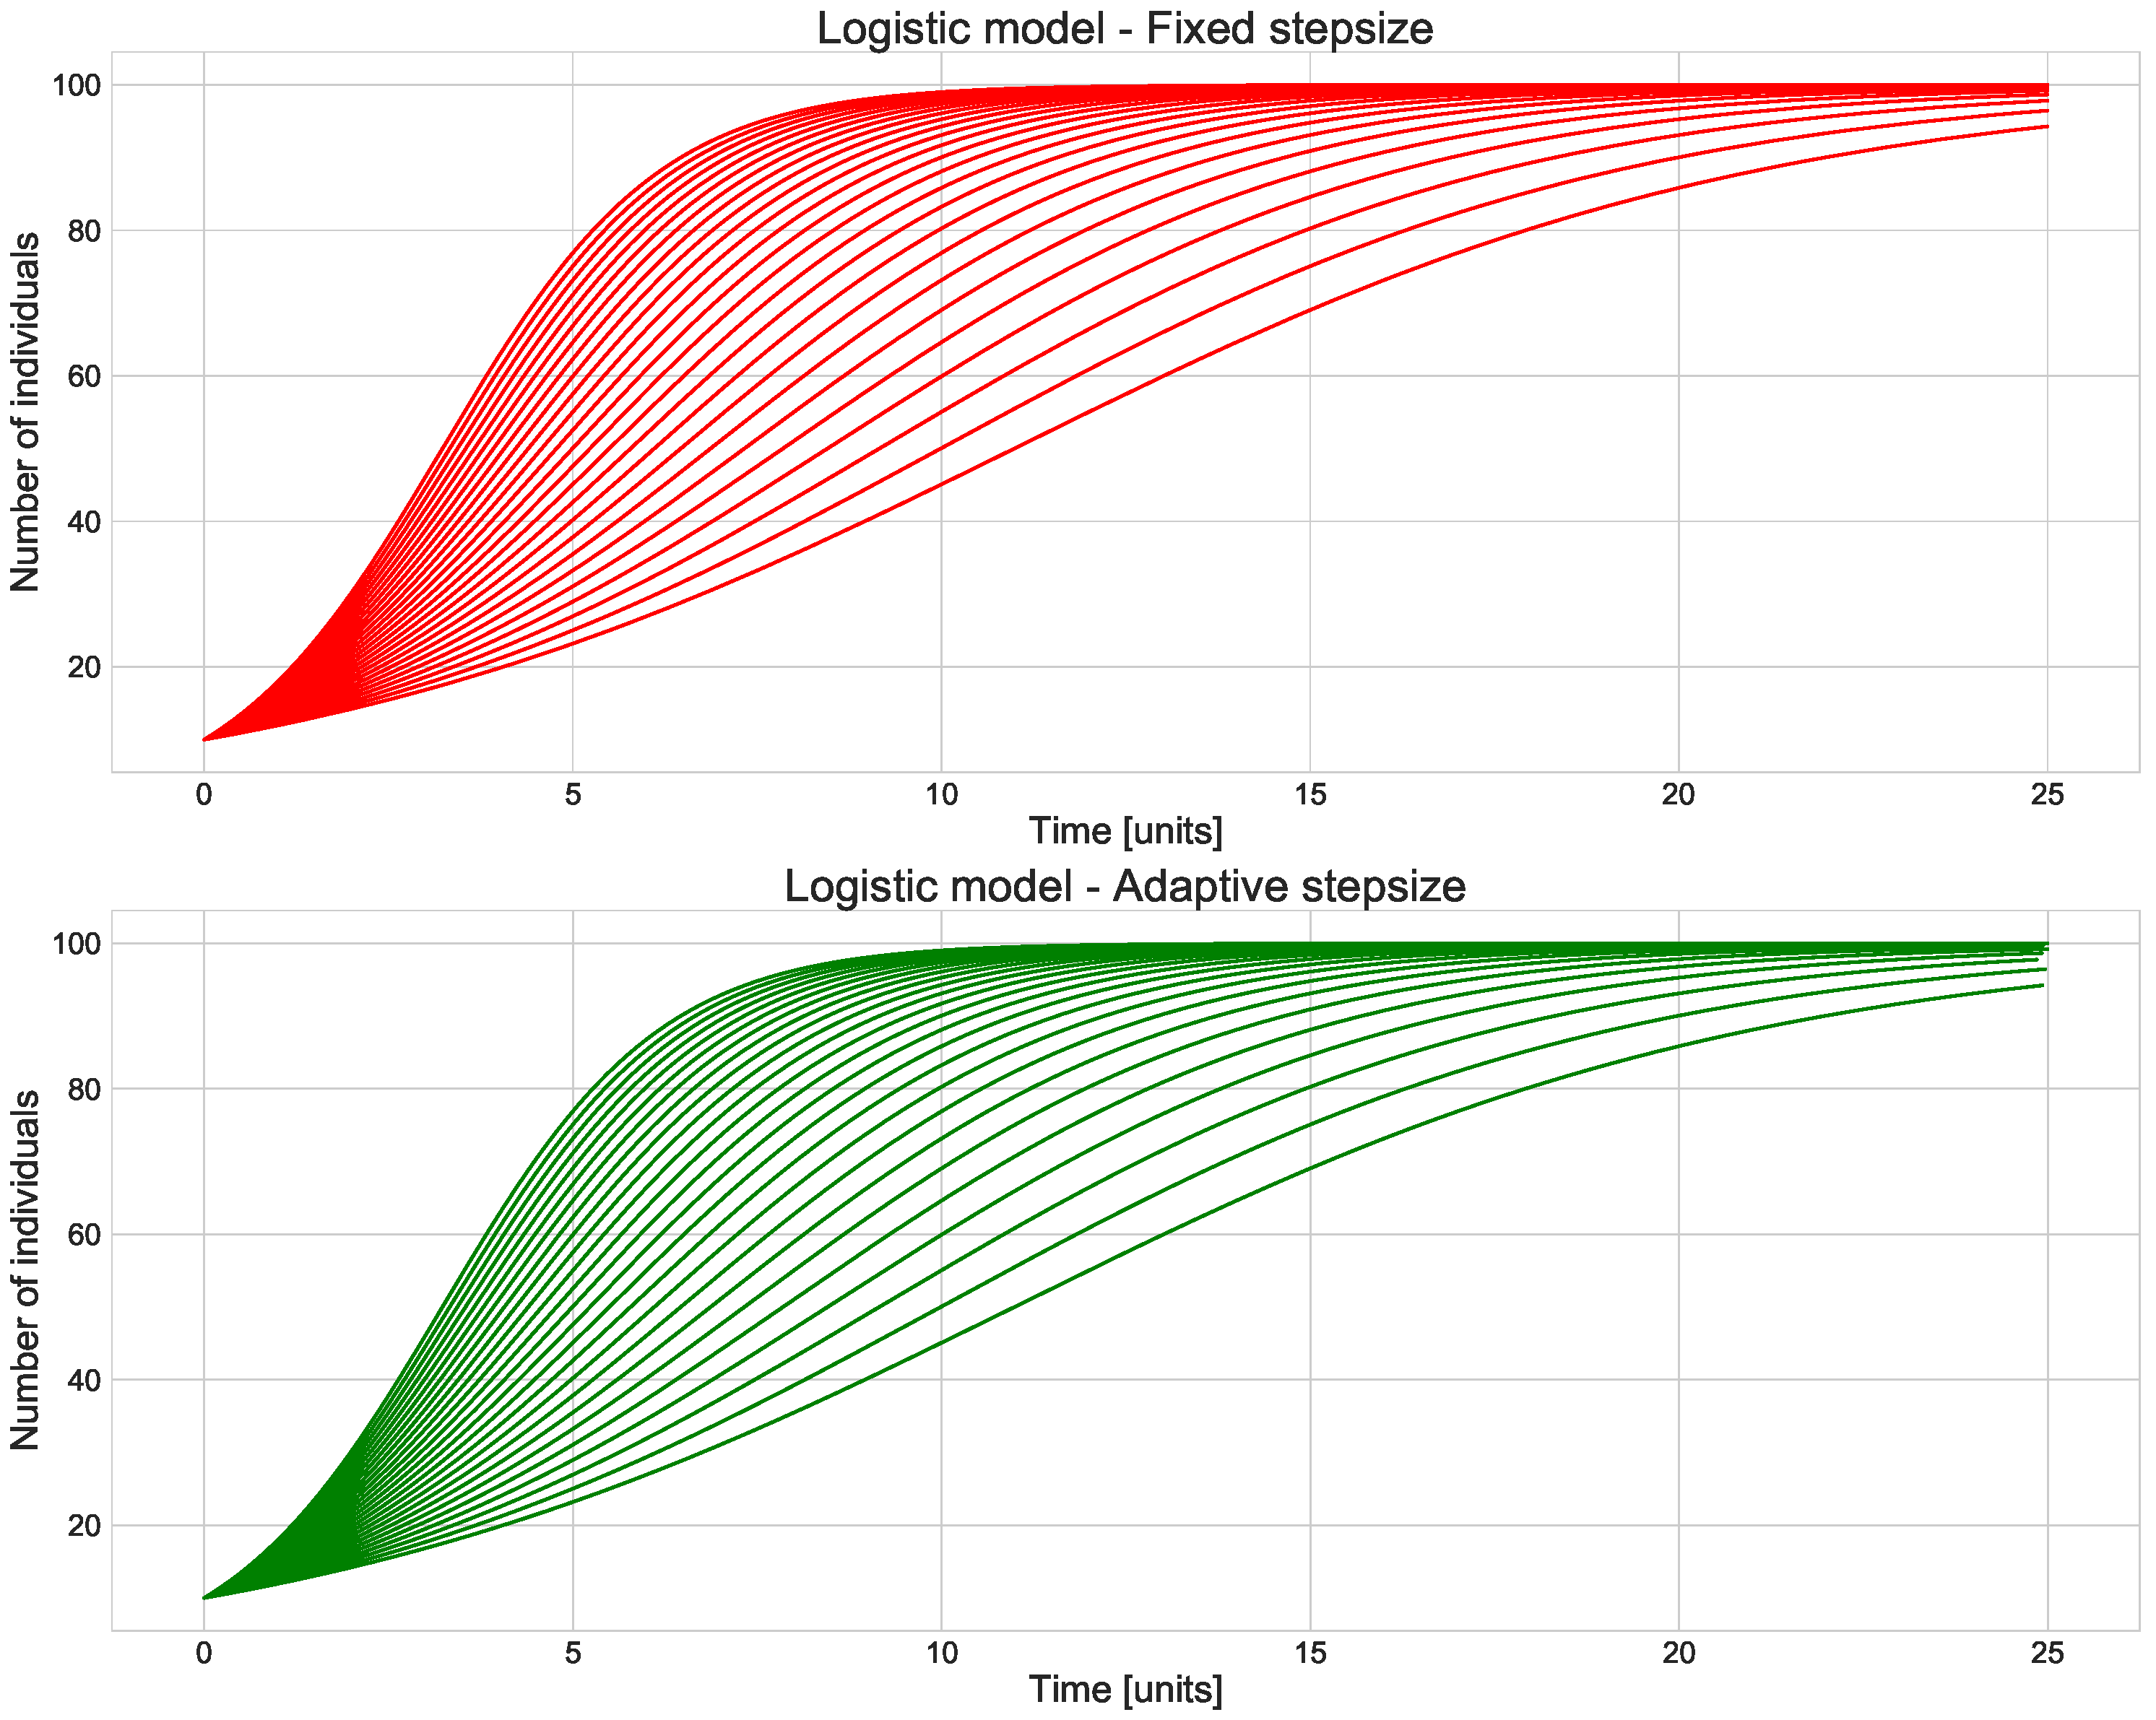
\includegraphics[width=0.95\textwidth]{images/logistic_model.pdf}
    \captionof{figure}{A logisztikus modell differenciálegyenletének megoldását adó egyik lehetséges görbesereg $w_{be} \in \left[ 0.5, 1 \right]$ születési rátára, $w_{ki} = 0.3$ halálozási ráta, $n_0 = 10$ kezdeti egyedszám és $k = 100$ maximális egyedszám mellett.} \label{fig:1}
\end{center}
\begin{center}
    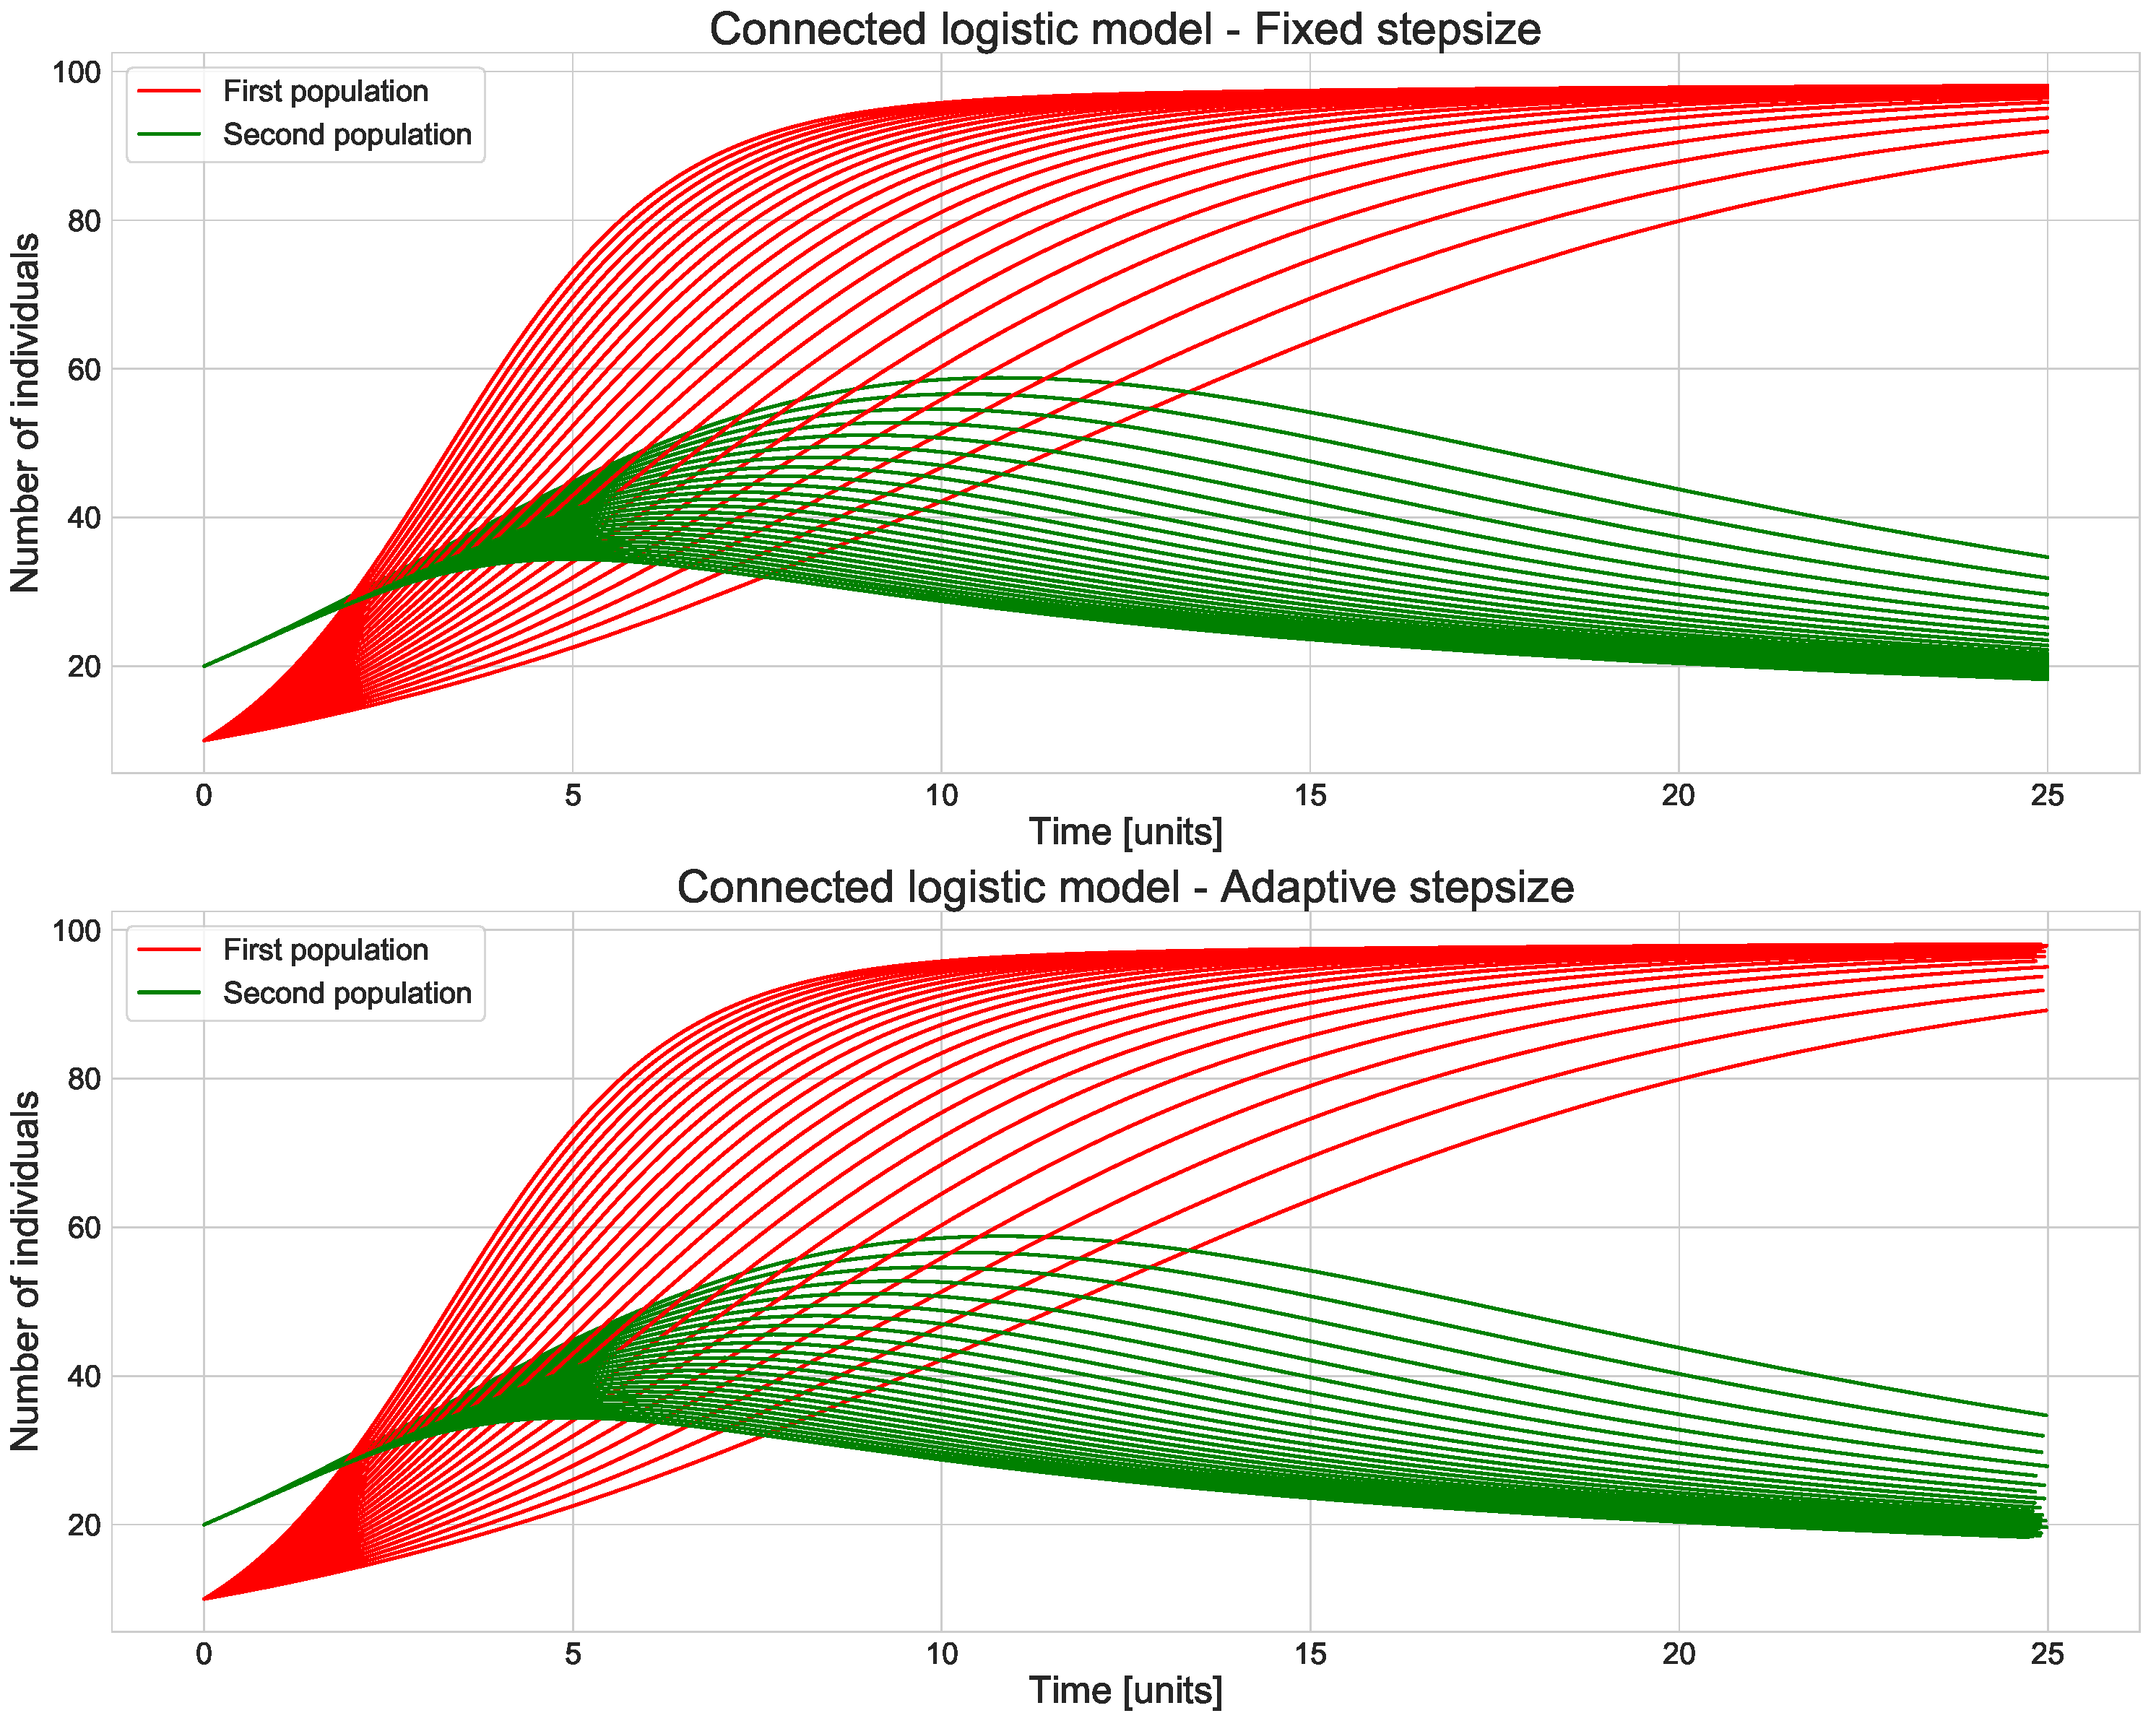
\includegraphics[width=0.95\textwidth]{images/connected_logistic_model.pdf}
    \captionof{figure}{A csatolt-logisztikus modell differenciálegyenletének megoldását adó egyik lehetséges görbesereg $w_{be_{1}} \in \left[ 0.5, 1 \right]$-re, ahol $w_{be_{1}}$ a sorszám szerinti első faj születési rátája, $w_{be_{2}} = 0.6$ születési, $w_{ki_{1}} = w_{ki_{2}} = 0.3$ halálozási ráták, $n_{0_{1}} = 10$, $n_{0_{2}} = 20$ kezdeti egyedszámok és $k_{1} = k_{2} = 100$ maximális egyedszám, valamint $\alpha = 0.1$ és $\beta = 0.9$ kölcsönhatási tényezők mellett.} \label{fig:2}
\end{center}
\vspace*{\fill}
\newpage
\topskip0pt
\vspace*{\fill}
\begin{center}
    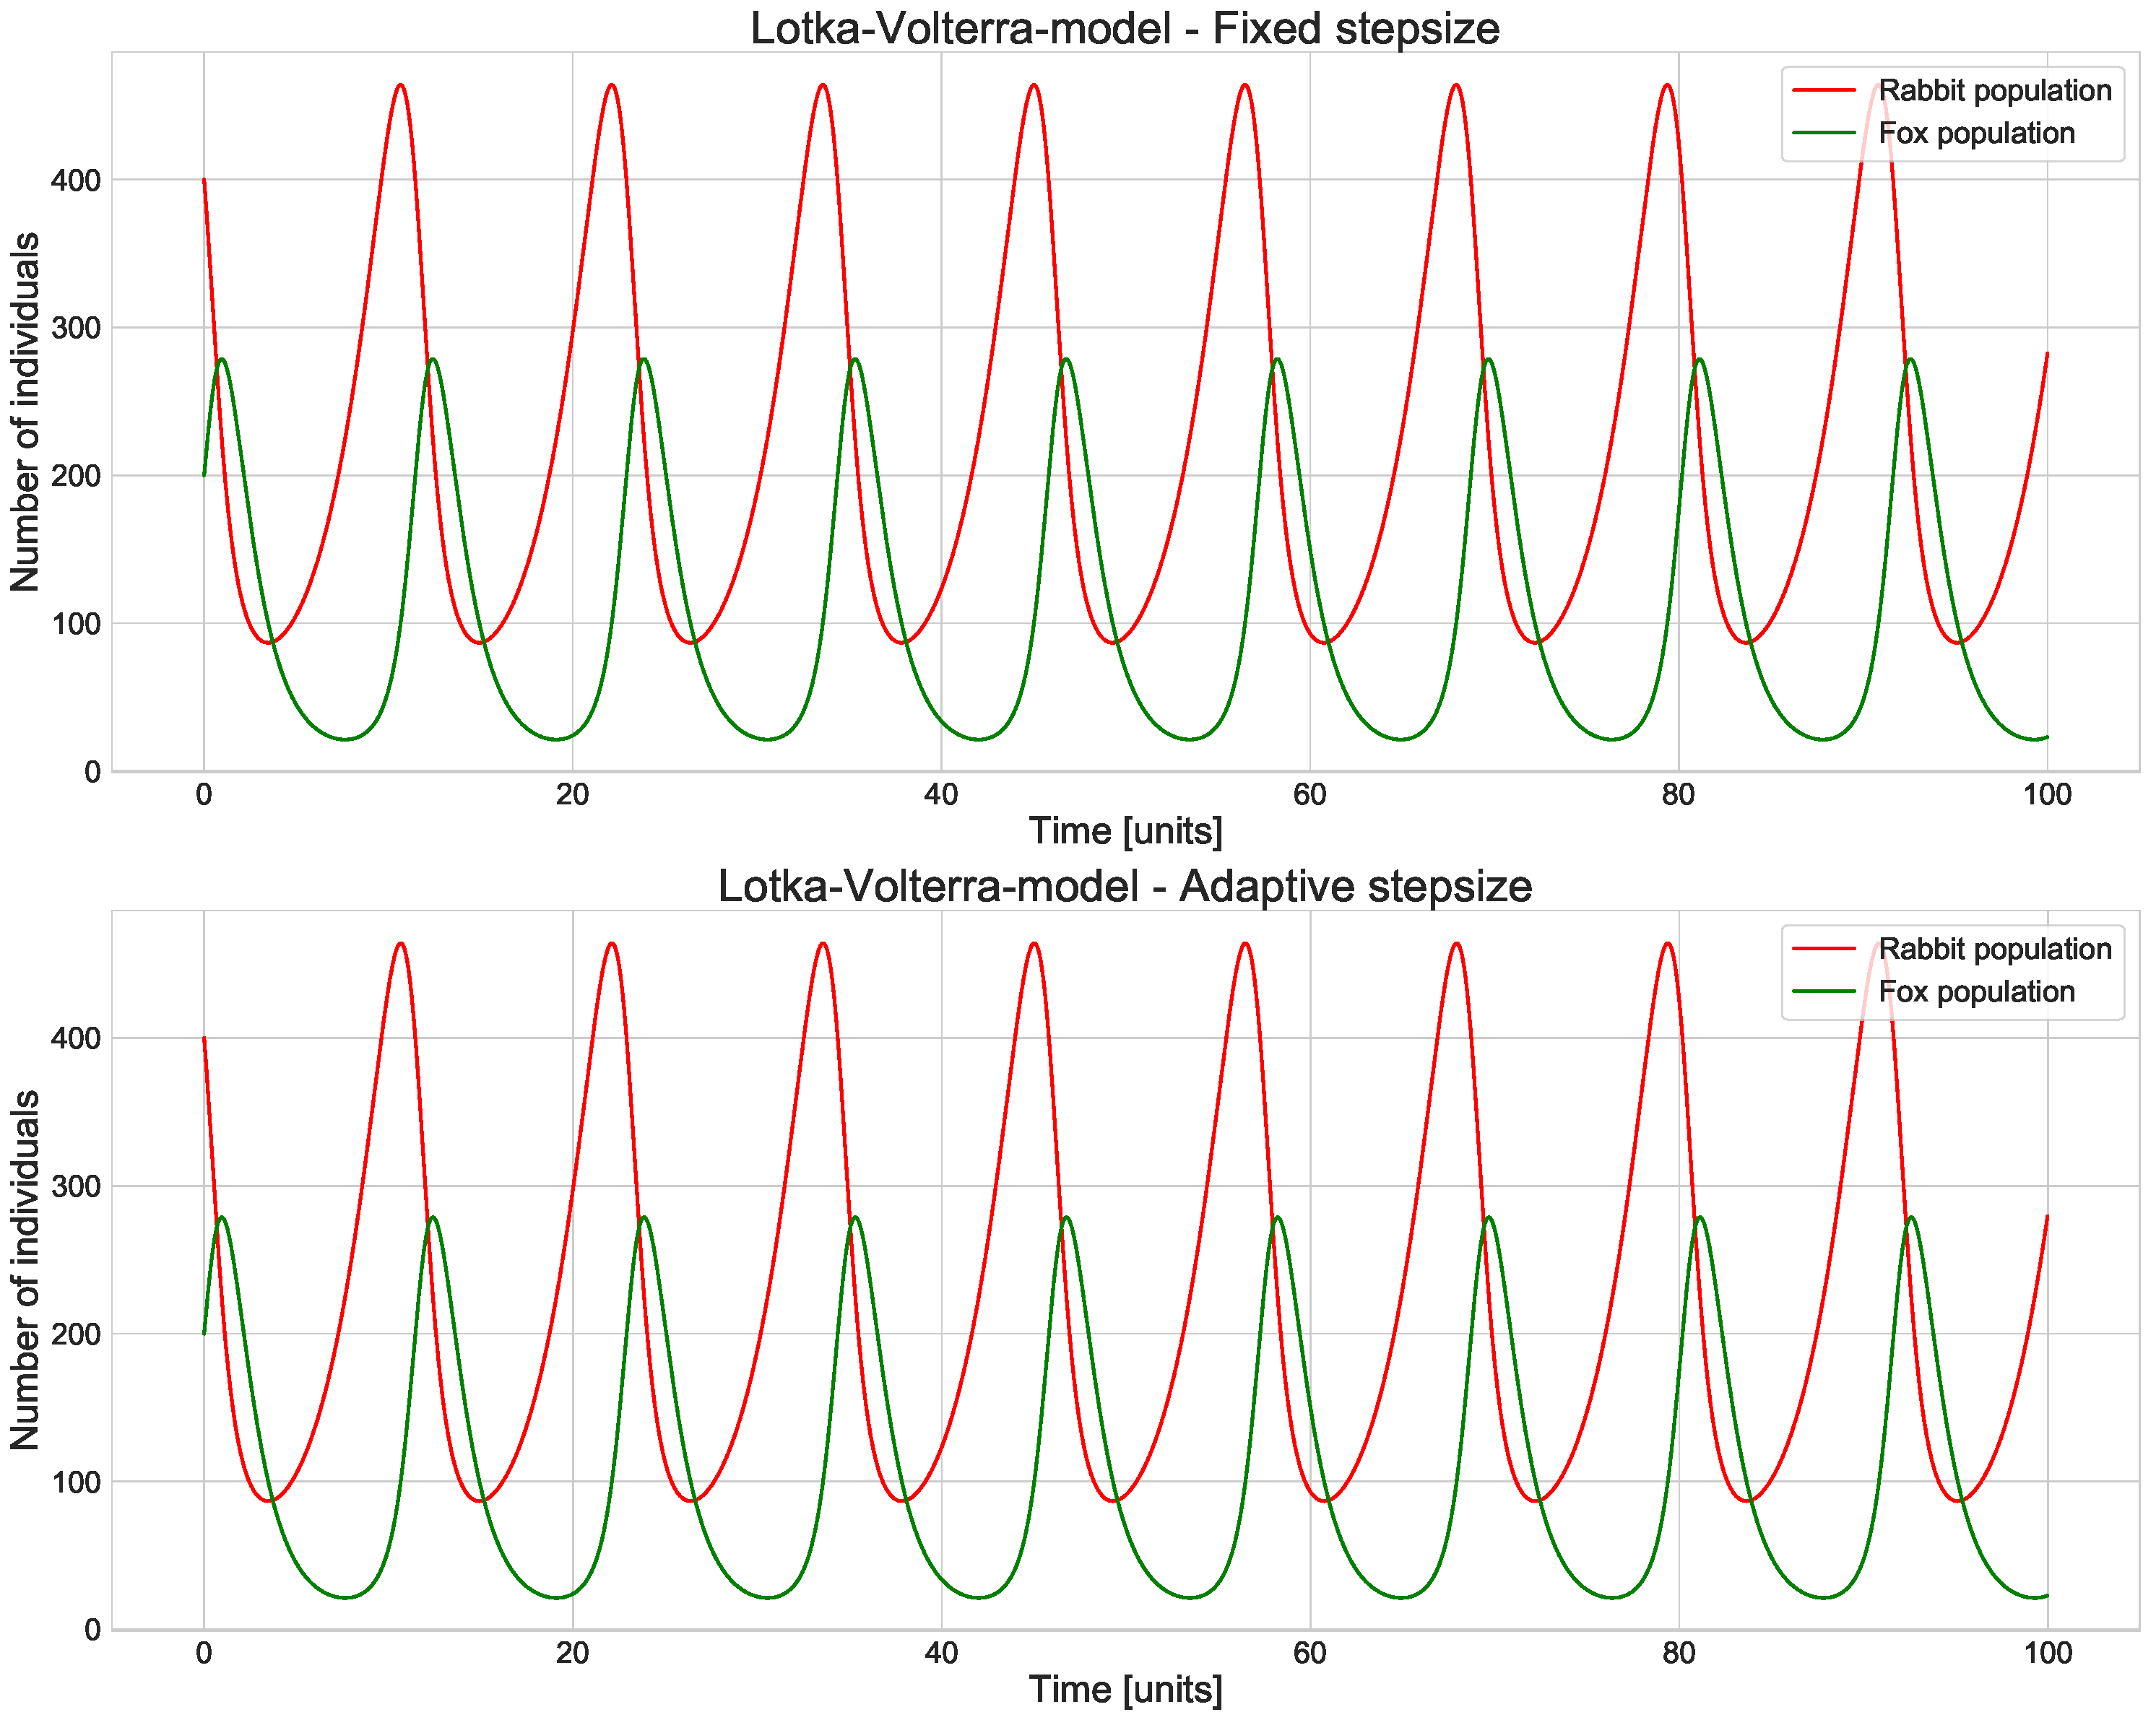
\includegraphics[width=\textwidth]{images/lv_model.pdf}
    \captionof{figure}{A Lotka--Volterra-modell differenciálegyenletének megoldását adó egyik lehetséges görbe, $n_{0_{r}} = 400$, $n_{0_{f}} = 200$ kezdeti egyedszámok, valamint $a = 0.4$, $b = c = 0.004$, $d = 0.9$ fejlődési ráták mellett, $k \to \infty$, $s = 0$ határesetben.} \label{fig:3}
\end{center}
\begin{center}
    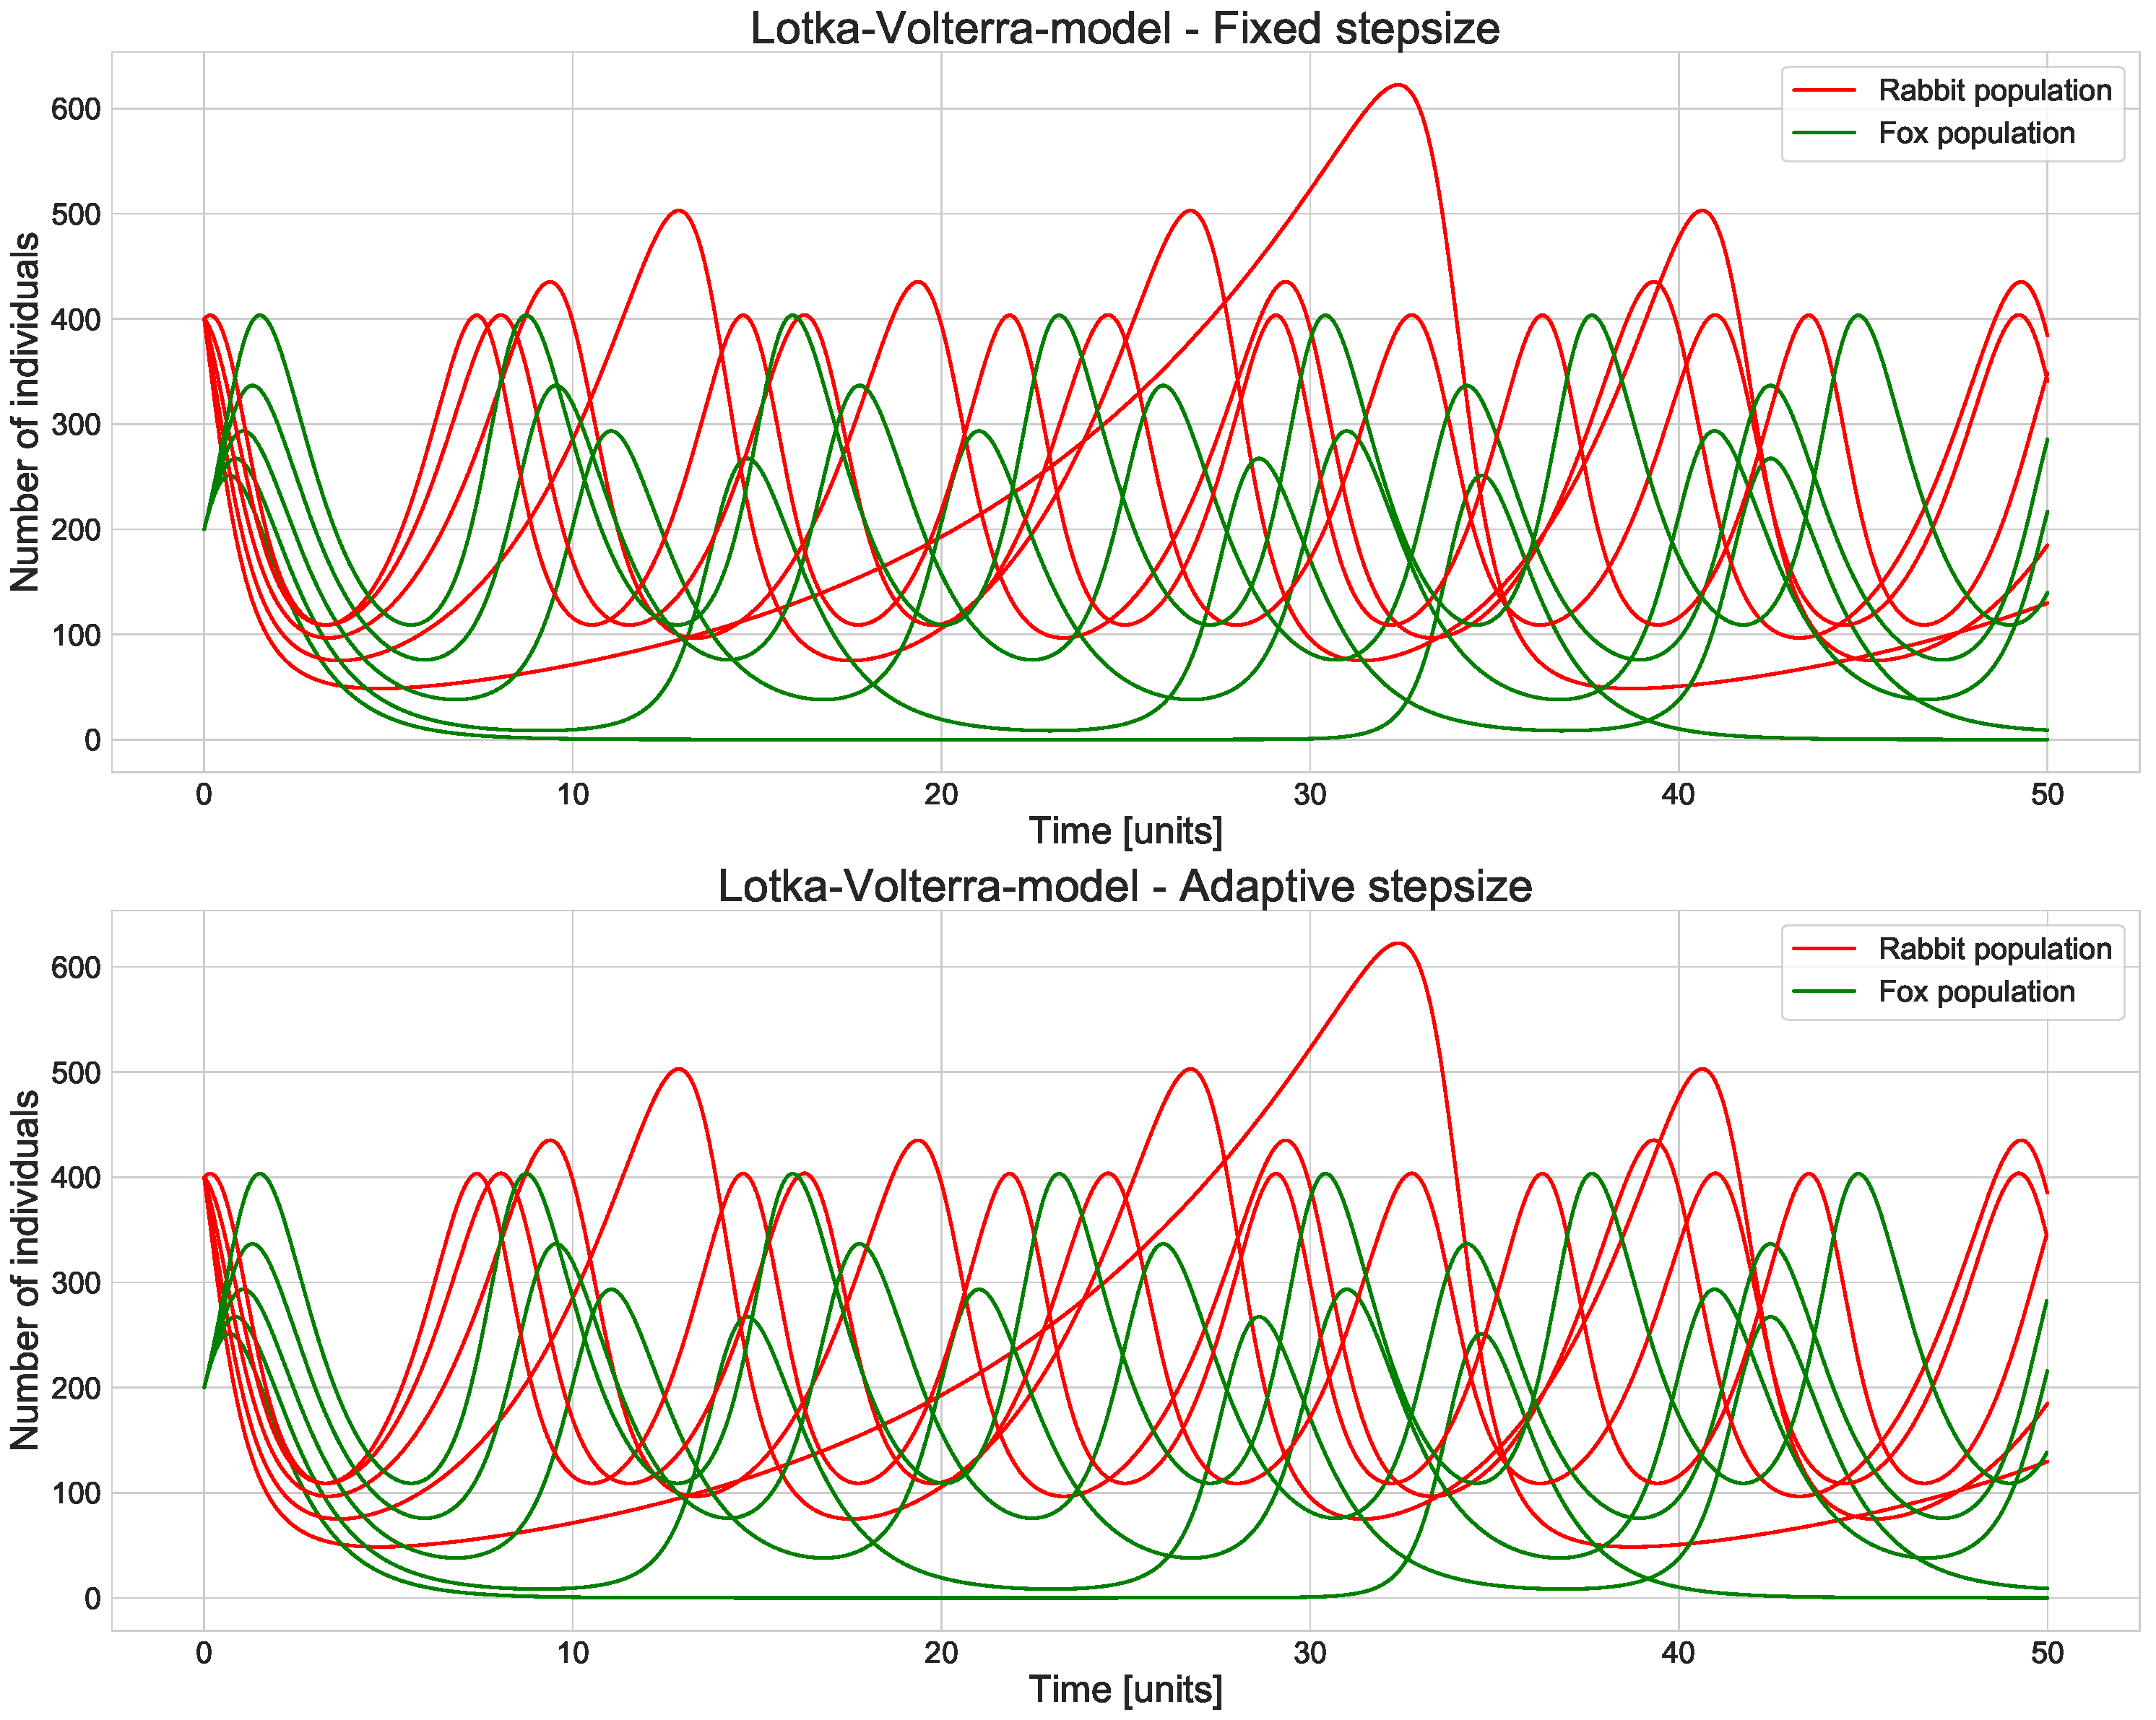
\includegraphics[width=\textwidth]{images/lv_model_more.pdf}
    \captionof{figure}{A Lotka--Volterra-modell differenciálegyenletének megoldását adó egyik lehetséges görbesereg, $a \in \left[ 0.1, 1.1 \right]$ paraméter esetén, $n_{0_{r}} = 400$, $n_{0_{f}} = 200$ kezdeti egyedszámok, valamint $b = c = 0.004$, $d = 0.9$ fejlődési ráták mellett, $k \to \infty$, $s = 0$ határesetben.} \label{fig:4}
\end{center}
\vspace*{\fill}
\newpage
\subsection*{A.2.  A logisztikus-modell stabilitásának vizsgálata az $r = -w_{ki} + w_{be}$ ráták arányának függvényében}
\topskip0pt
\vspace*{\fill}
\begin{center}
    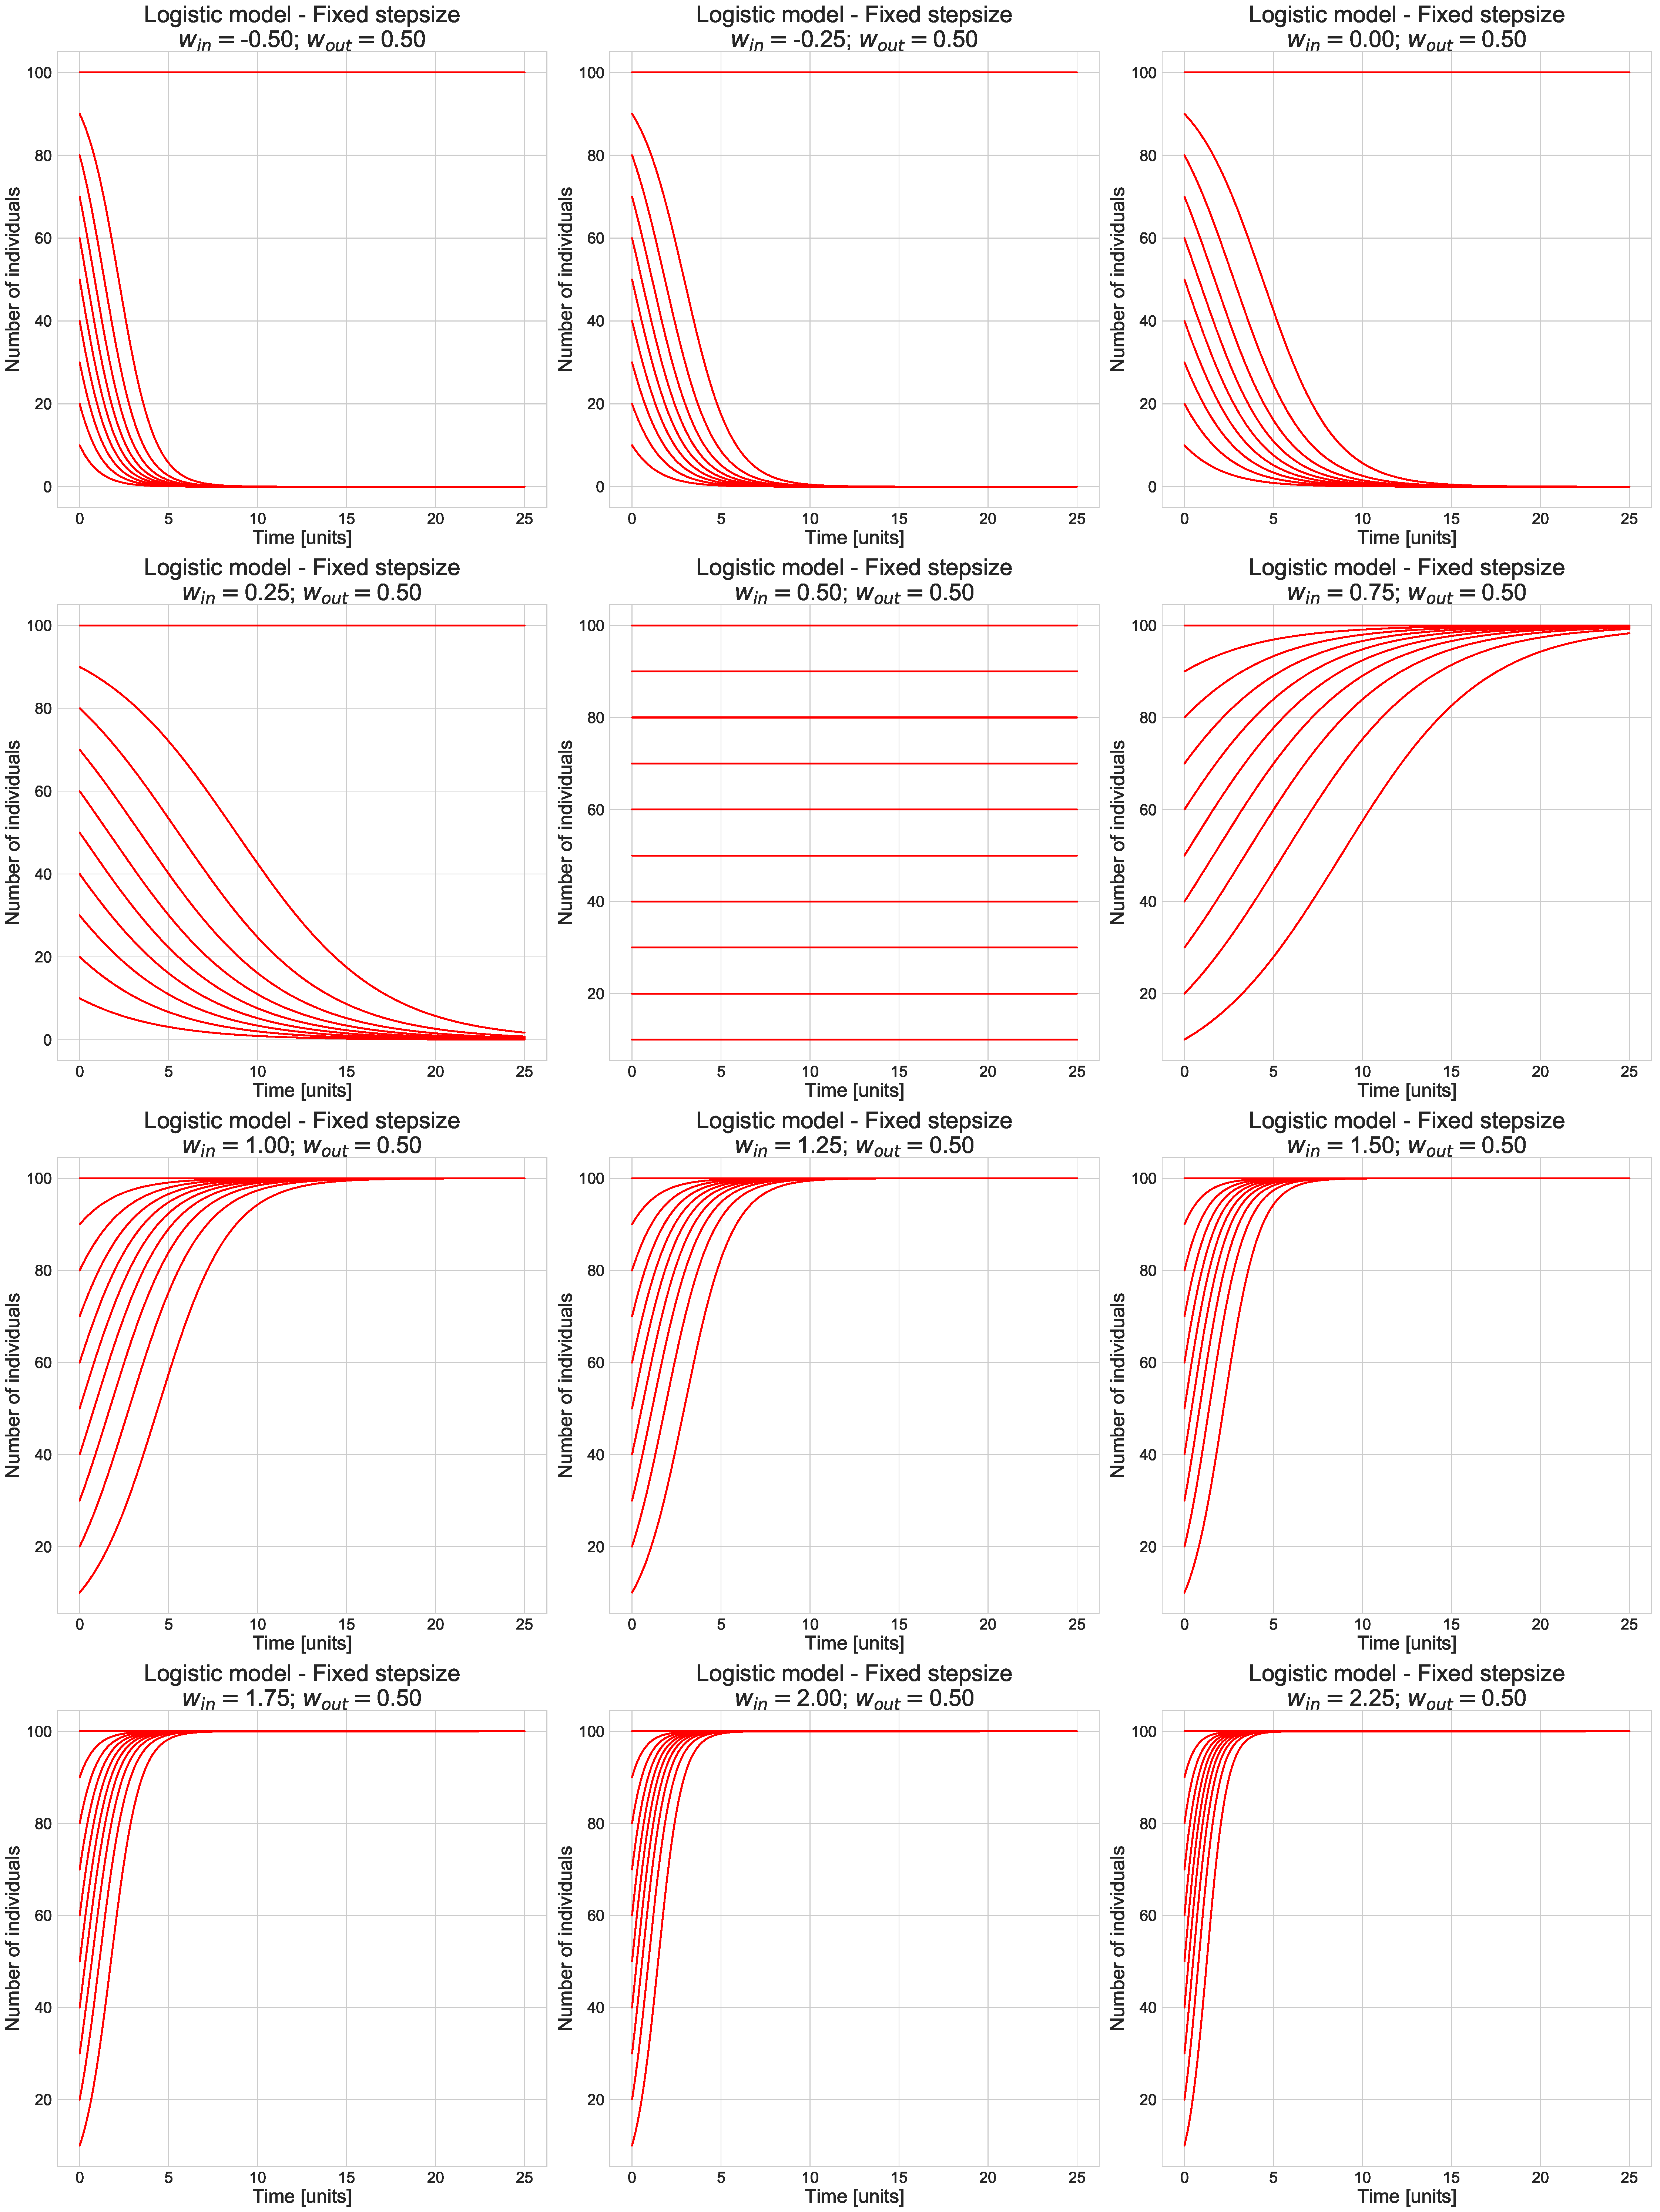
\includegraphics[width=\textwidth]{images/logistic_model_numerous.pdf}
    \captionof{figure}{A logisztikus-modell stabilitásának vizsgálata, $w_{be} \in \left[ -0.5, 2.25 \right]$ születési, $w_{ki} = 0.5$ halálozás ráták mellett, minden egyes $r$ érték esetén $n_{0} \in \left[ 10, 100 \right]$ kezdeti egyedszám és $k = 100$ maximális egyedszám esetében.} \label{fig:5}
\end{center}
\vspace*{\fill}
\newpage
\topskip0pt
\vspace*{\fill}
\begin{center}
    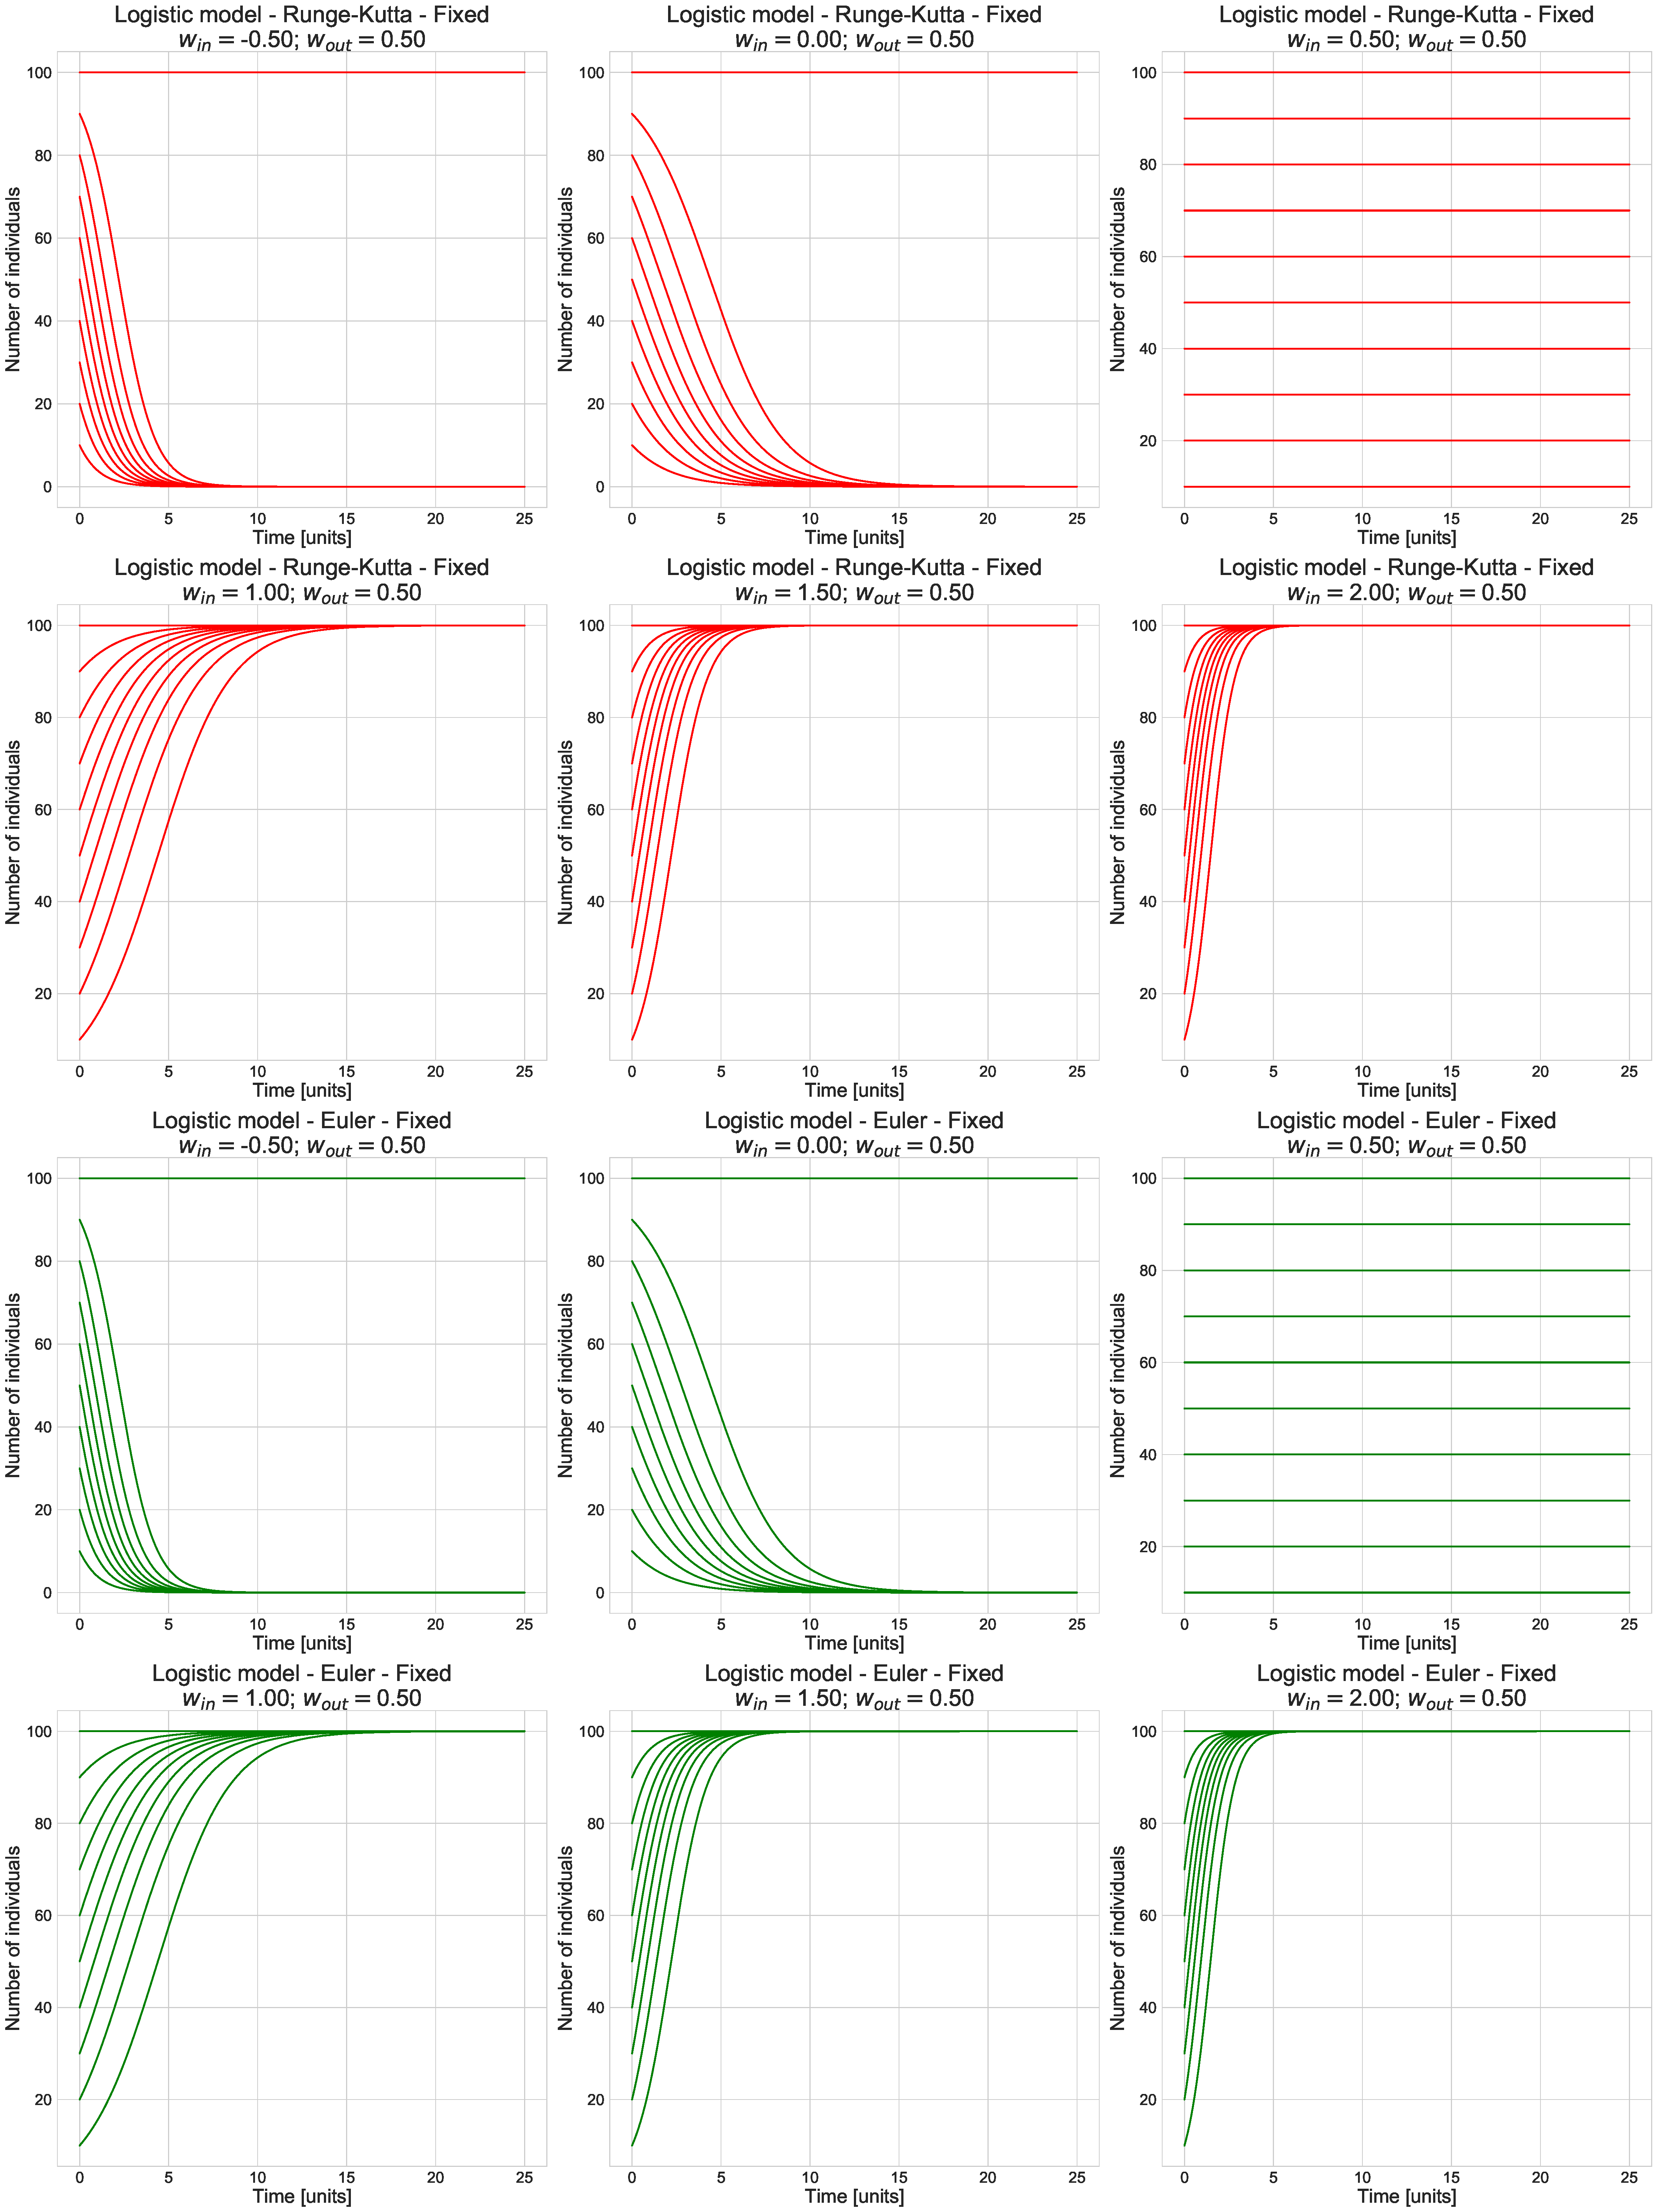
\includegraphics[width=\textwidth]{images/logistic_model_compare_odeints.pdf}
    \captionof{figure}{A logisztikus-modell stabilitásának vizsgálata és az Euler-, valamint negyedrendű Runge--Kutta-módszerek összehasonlítása, $w_{be} \in \left[ -0.5, 2 \right]$ születési, $w_{ki} = 0.5$ halálozás ráták mellett, minden egyes $r$ érték esetén $n_{0} \in \left[ 10, 100 \right]$ kezdeti egyedszám és $k = 100$ maximális egyedszám esetében. A felső 6 grafikon a negyedrendű Runge--Kutta módszerrel integrált görbeseregeket, míg az alsó 6 az Euler-módszer segítségével integráltakat mutatja.} \label{fig:6}
\end{center}
\vspace*{\fill}
\newpage
\topskip0pt
\vspace*{\fill}
\begin{center}
    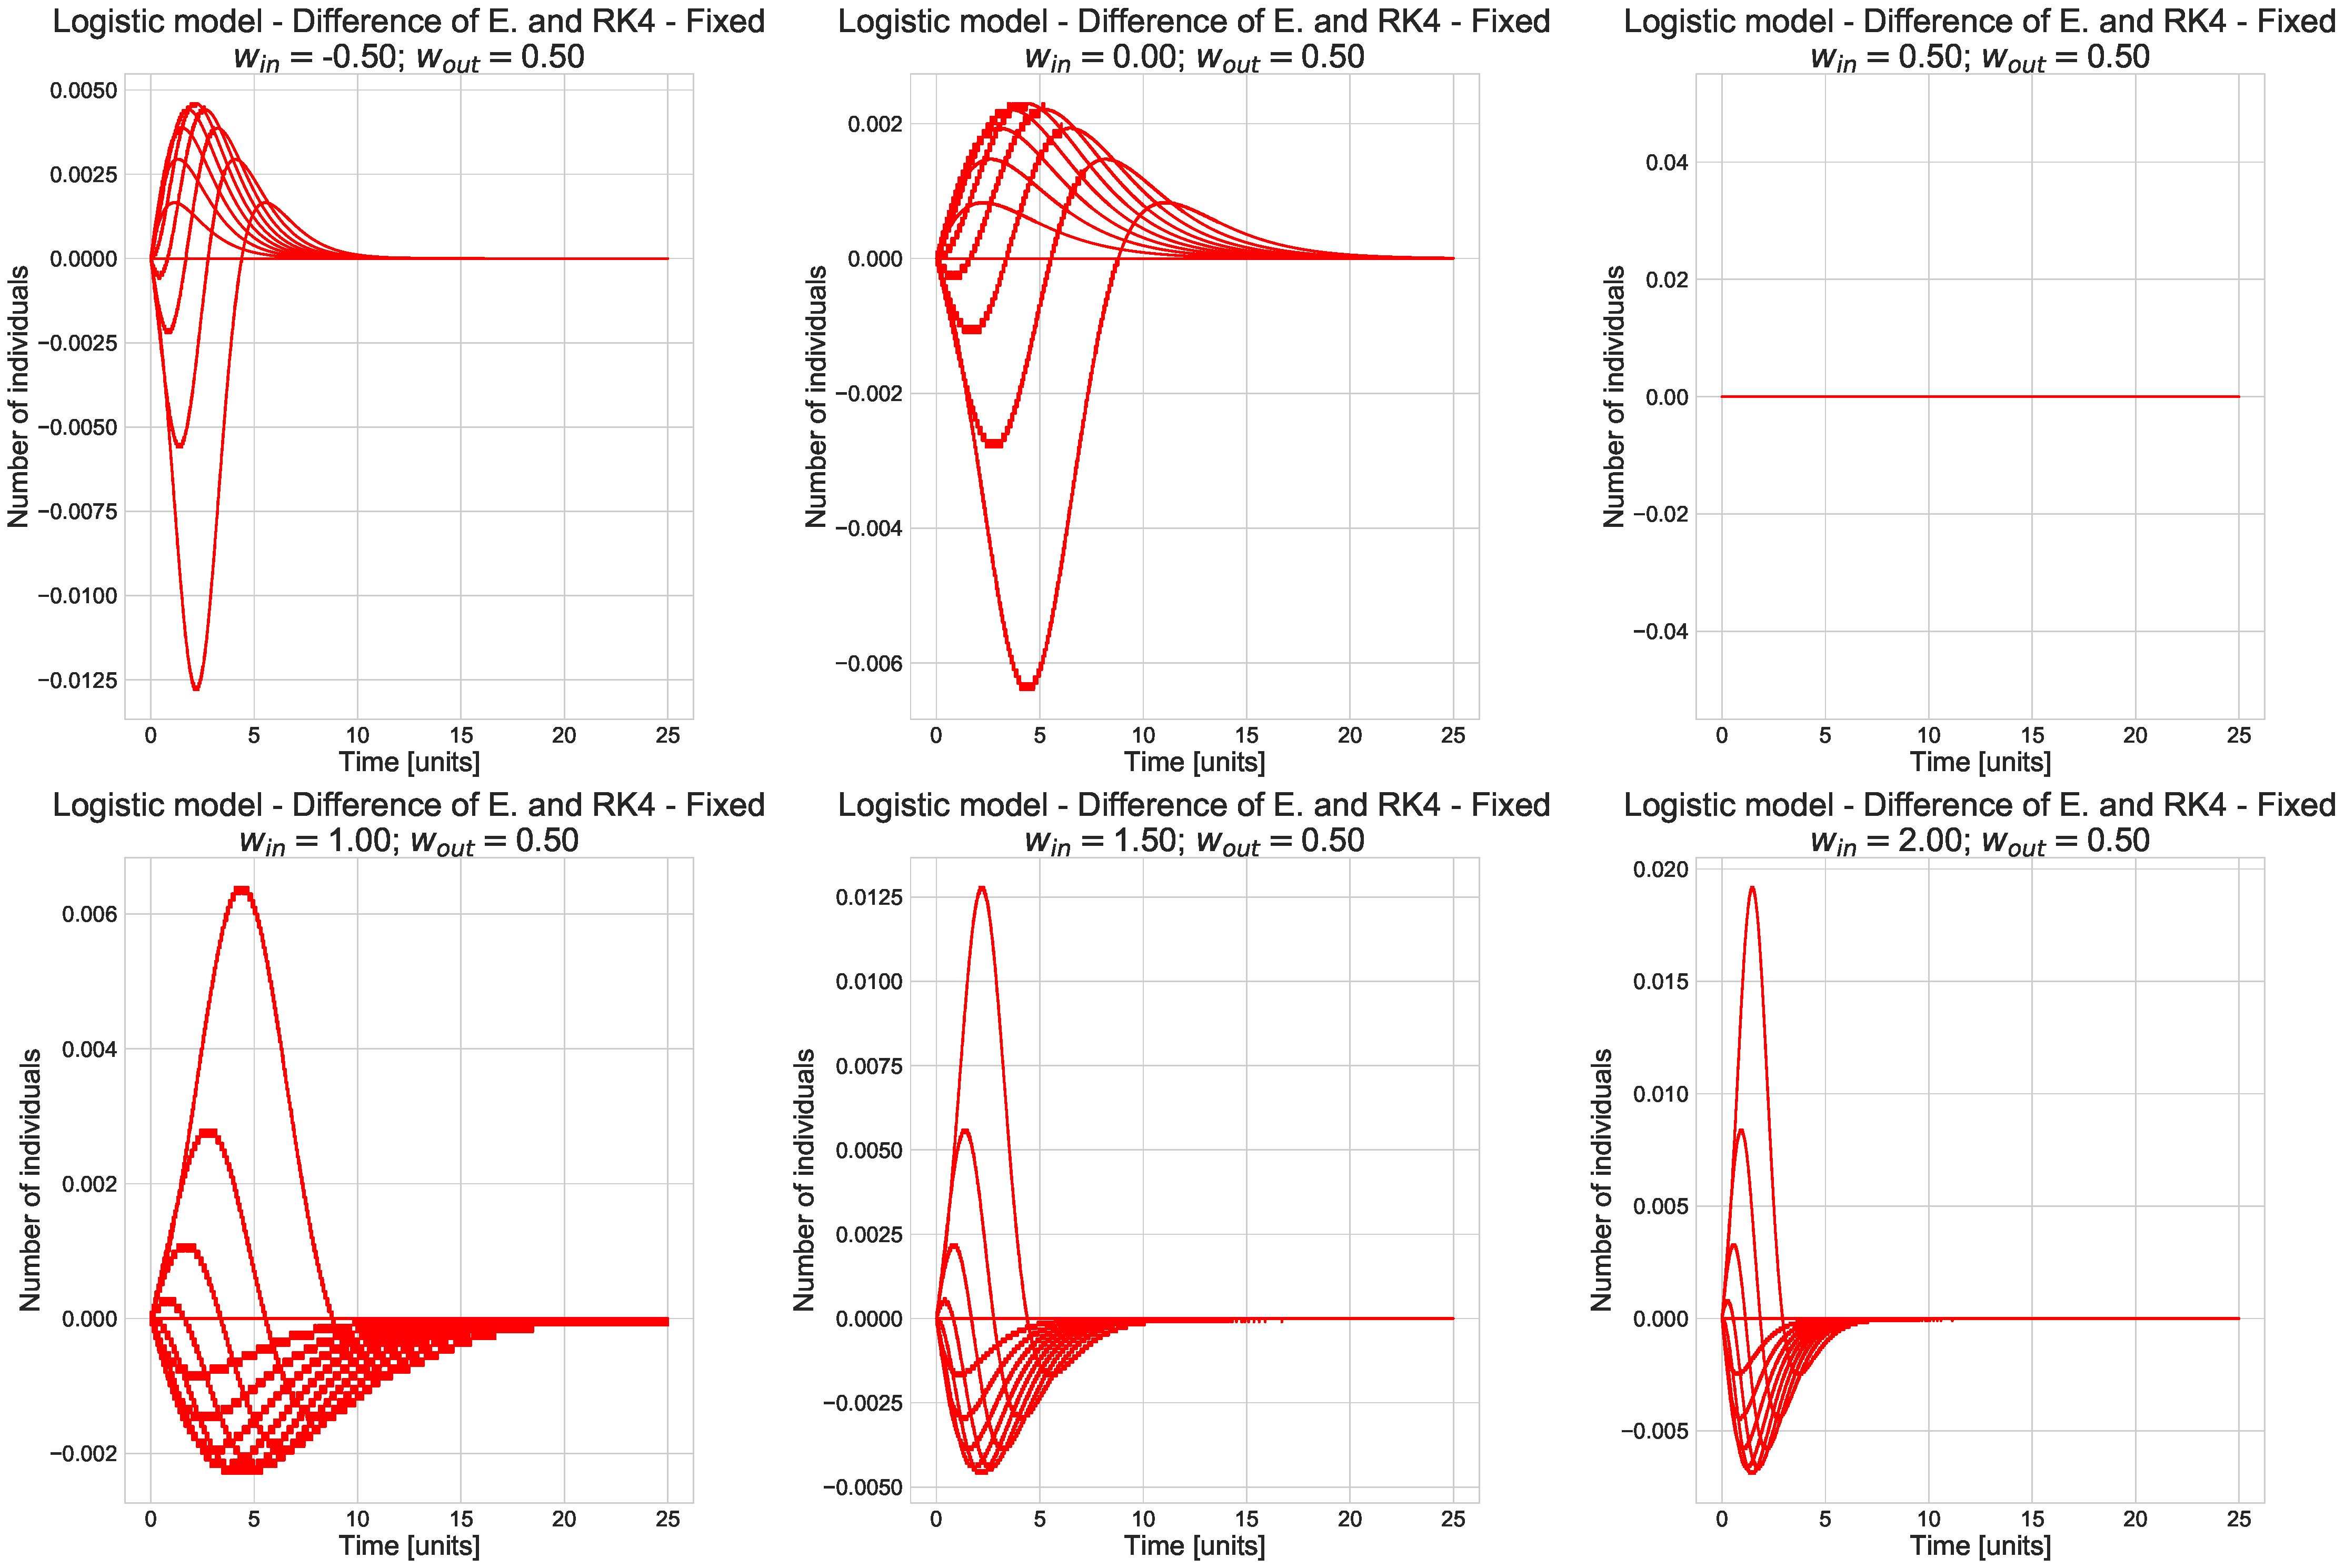
\includegraphics[width=\textwidth]{images/logistic_model_compare_odeints_diff.pdf}
    \captionof{figure}{A logisztikus-modell stabilitásának vizsgálata és az Euler-, valamint negyedrendű Runge--Kutta-módszerek előző ábrán szereplő értékeinek különbsége, $w_{be} \in \left[ -0.5, 2 \right]$ születési, $w_{ki} = 0.5$ halálozás ráták mellett, minden egyes $r$ érték esetén $n_{0} \in \left[ 10, 100 \right]$ kezdeti egyedszám és $k = 100$ maximális egyedszám esetében.} \label{fig:7}
\end{center}
\begin{center}
    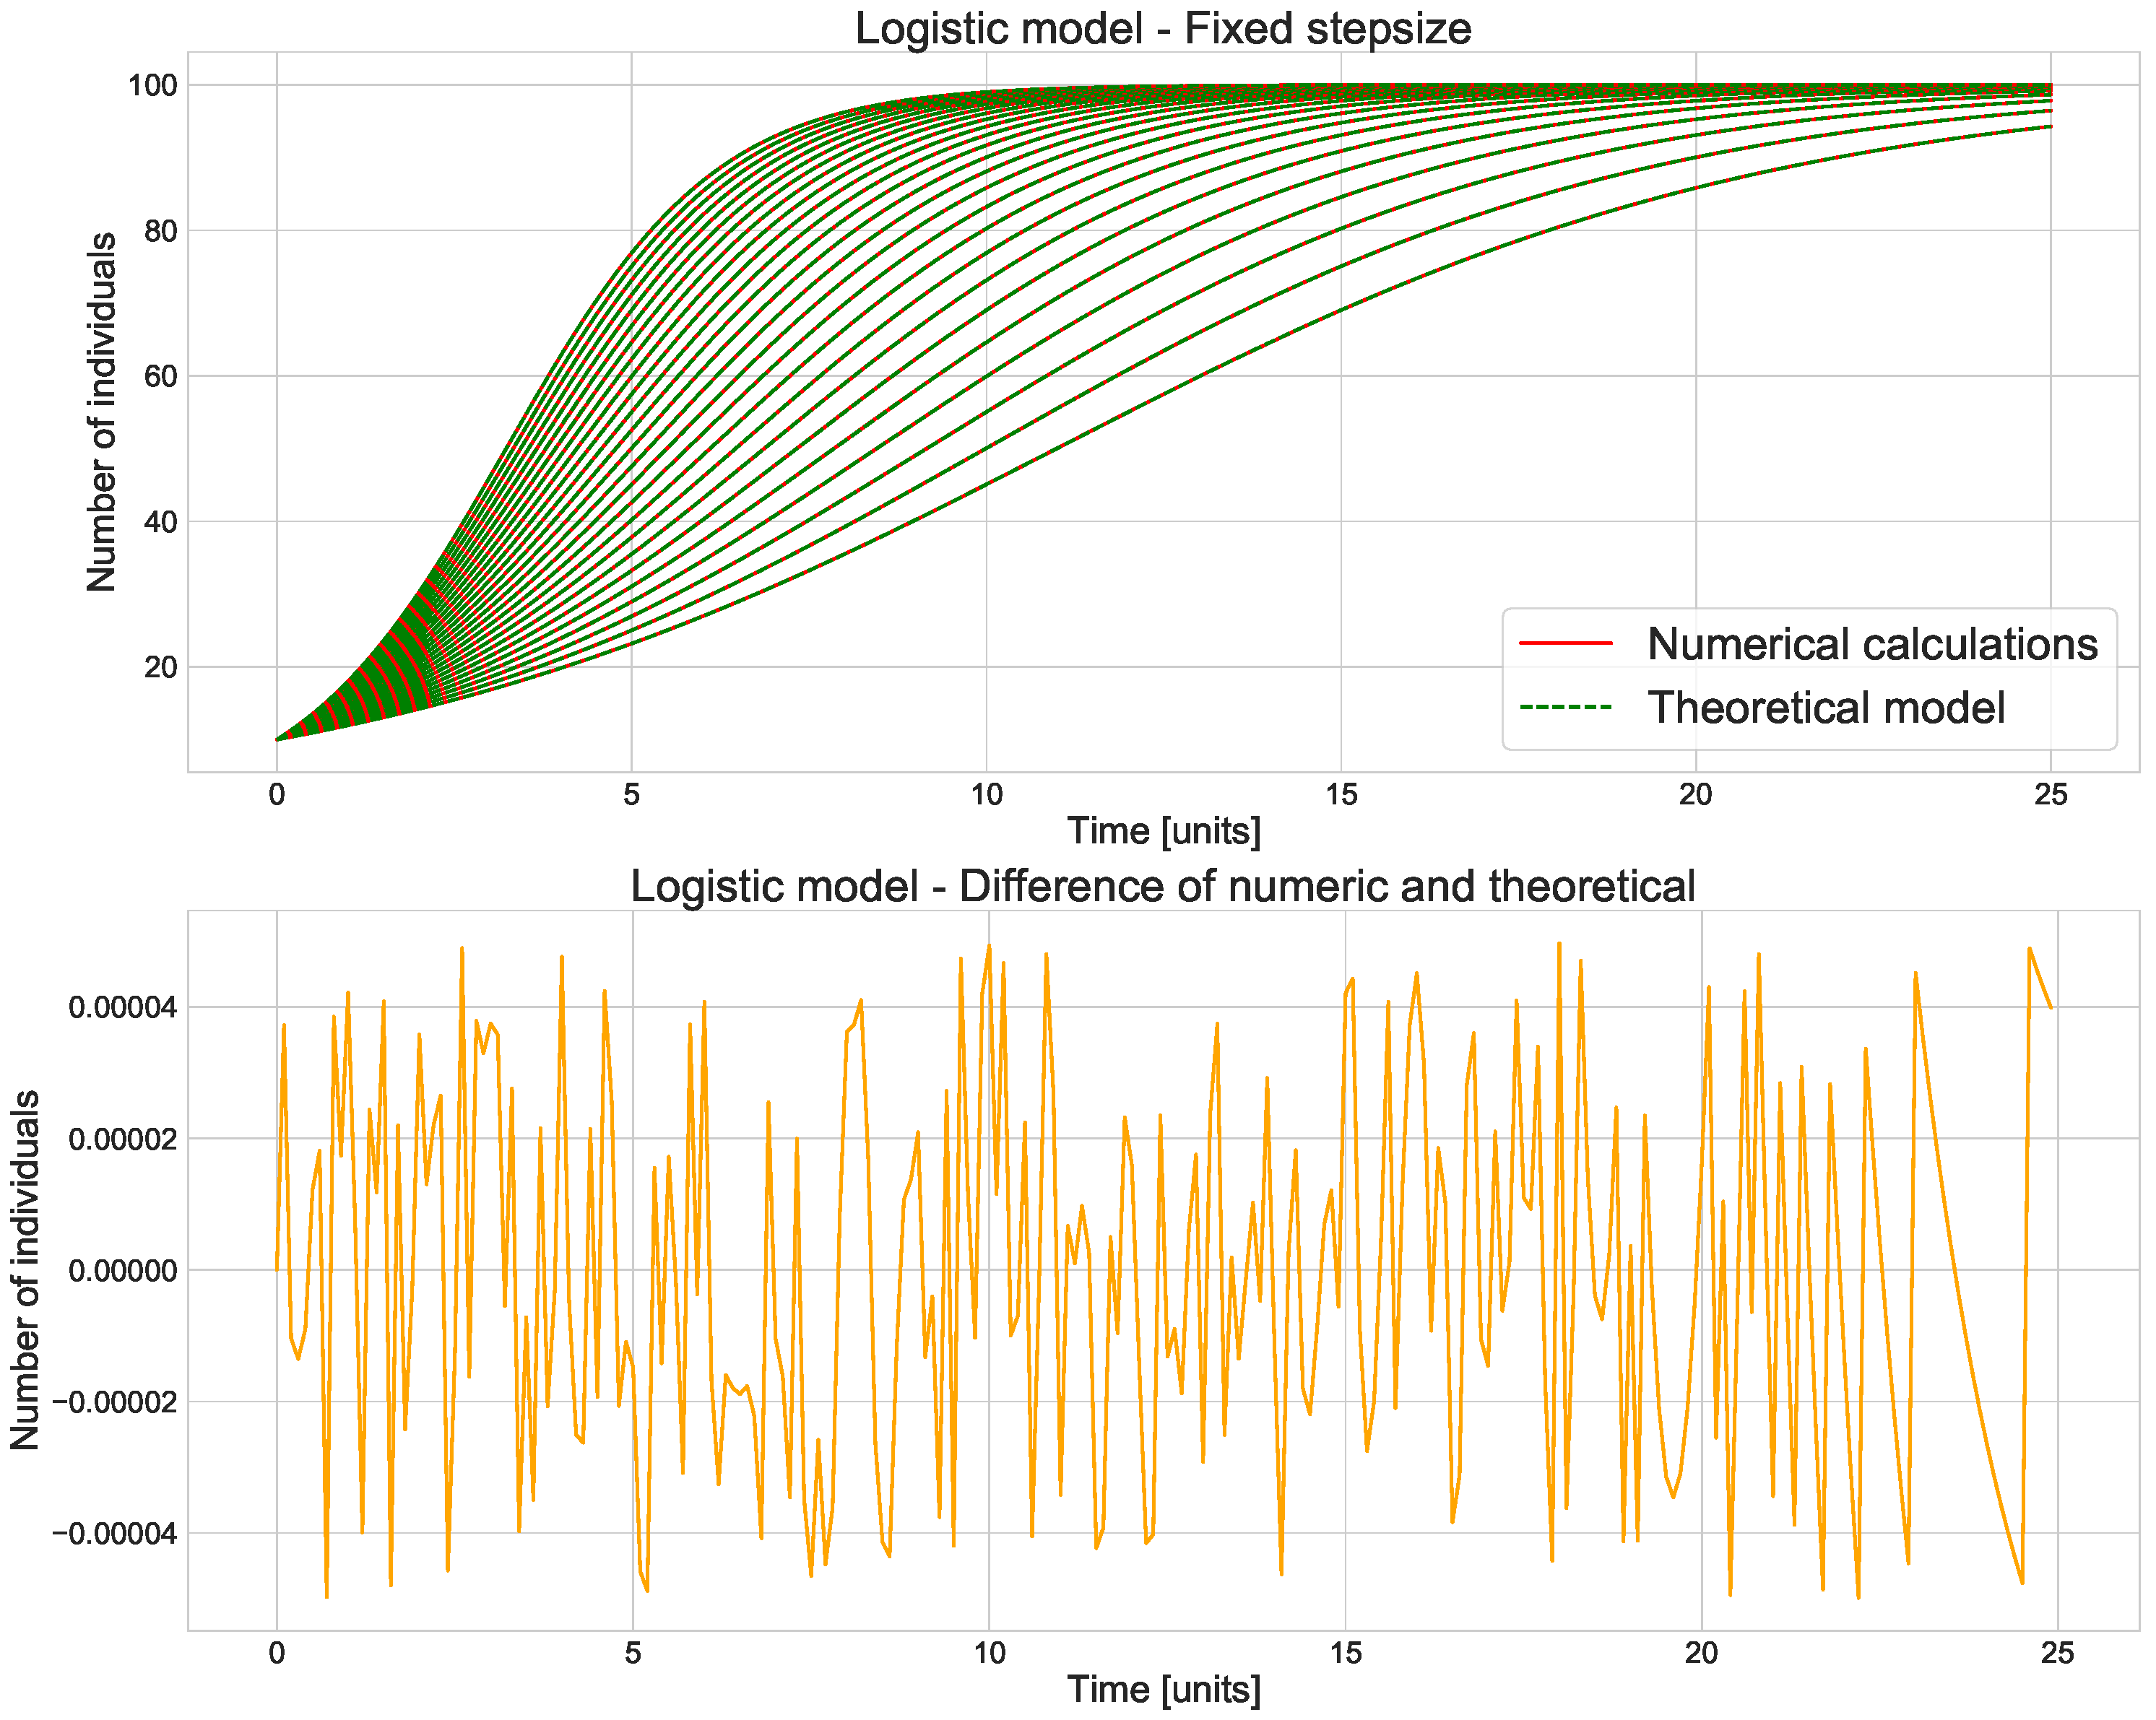
\includegraphics[width=\textwidth]{images/logistic_model_compare_theory.pdf}
    \captionof{figure}{A logisztikus-modell numerikus és elméleti eredményeinek összehasonlítása, $w_{be} \in \left[ 0.5, 1 \right]$ születési, $w_{ki} = 0.3$ halálozás ráták mellett, minden egyes $r$ érték esetén $n_{0} = 10$ kezdeti egyedszám és $k = 100$ maximális egyedszám esetében. Az alsó kép szemmel láthatóan magyarázatot igényel. Ezen a felette látható grafikonon található görbék közüli legutolsóhoz ($w_{ki} = 1$) tartozó numerikus és elméleti eredmény különbségét ábrázoltam. A kép minden egyes görbére hasonló, zajra emlékeztető viselkedést mutatott. A jobb átláthatóság kedvéért az egyetlen ábrázolt görbének csak minden 100. pontját jelenítettem meg a grafikonon. Erről az olvasható le, hogy az elméletitől való eltérés szinte minden lépésben, két szélső pont között ugrál (jelen képen ezek kb. a $\pm 0.00004$ értékek). A kapott eredmény mindenképp elgondolkodtató és egyértelműen valamilyen szisztematikus numerikus hibát jelent. Mivel a numerikus eredményt a Runge--Kutta--Cash--Karp-módszer felhasználásával készítettem, így a hiba mindenképp abban keresendő.} \label{fig:8}
\end{center}
\vspace*{\fill}
\newpage
\subsection*{A.3.  A csatolt-logisztikus-modell stabilitásának vizsgálata a $k$ maximális egyedszám függvényében}
\topskip0pt
\vspace*{\fill}
\begin{center}
    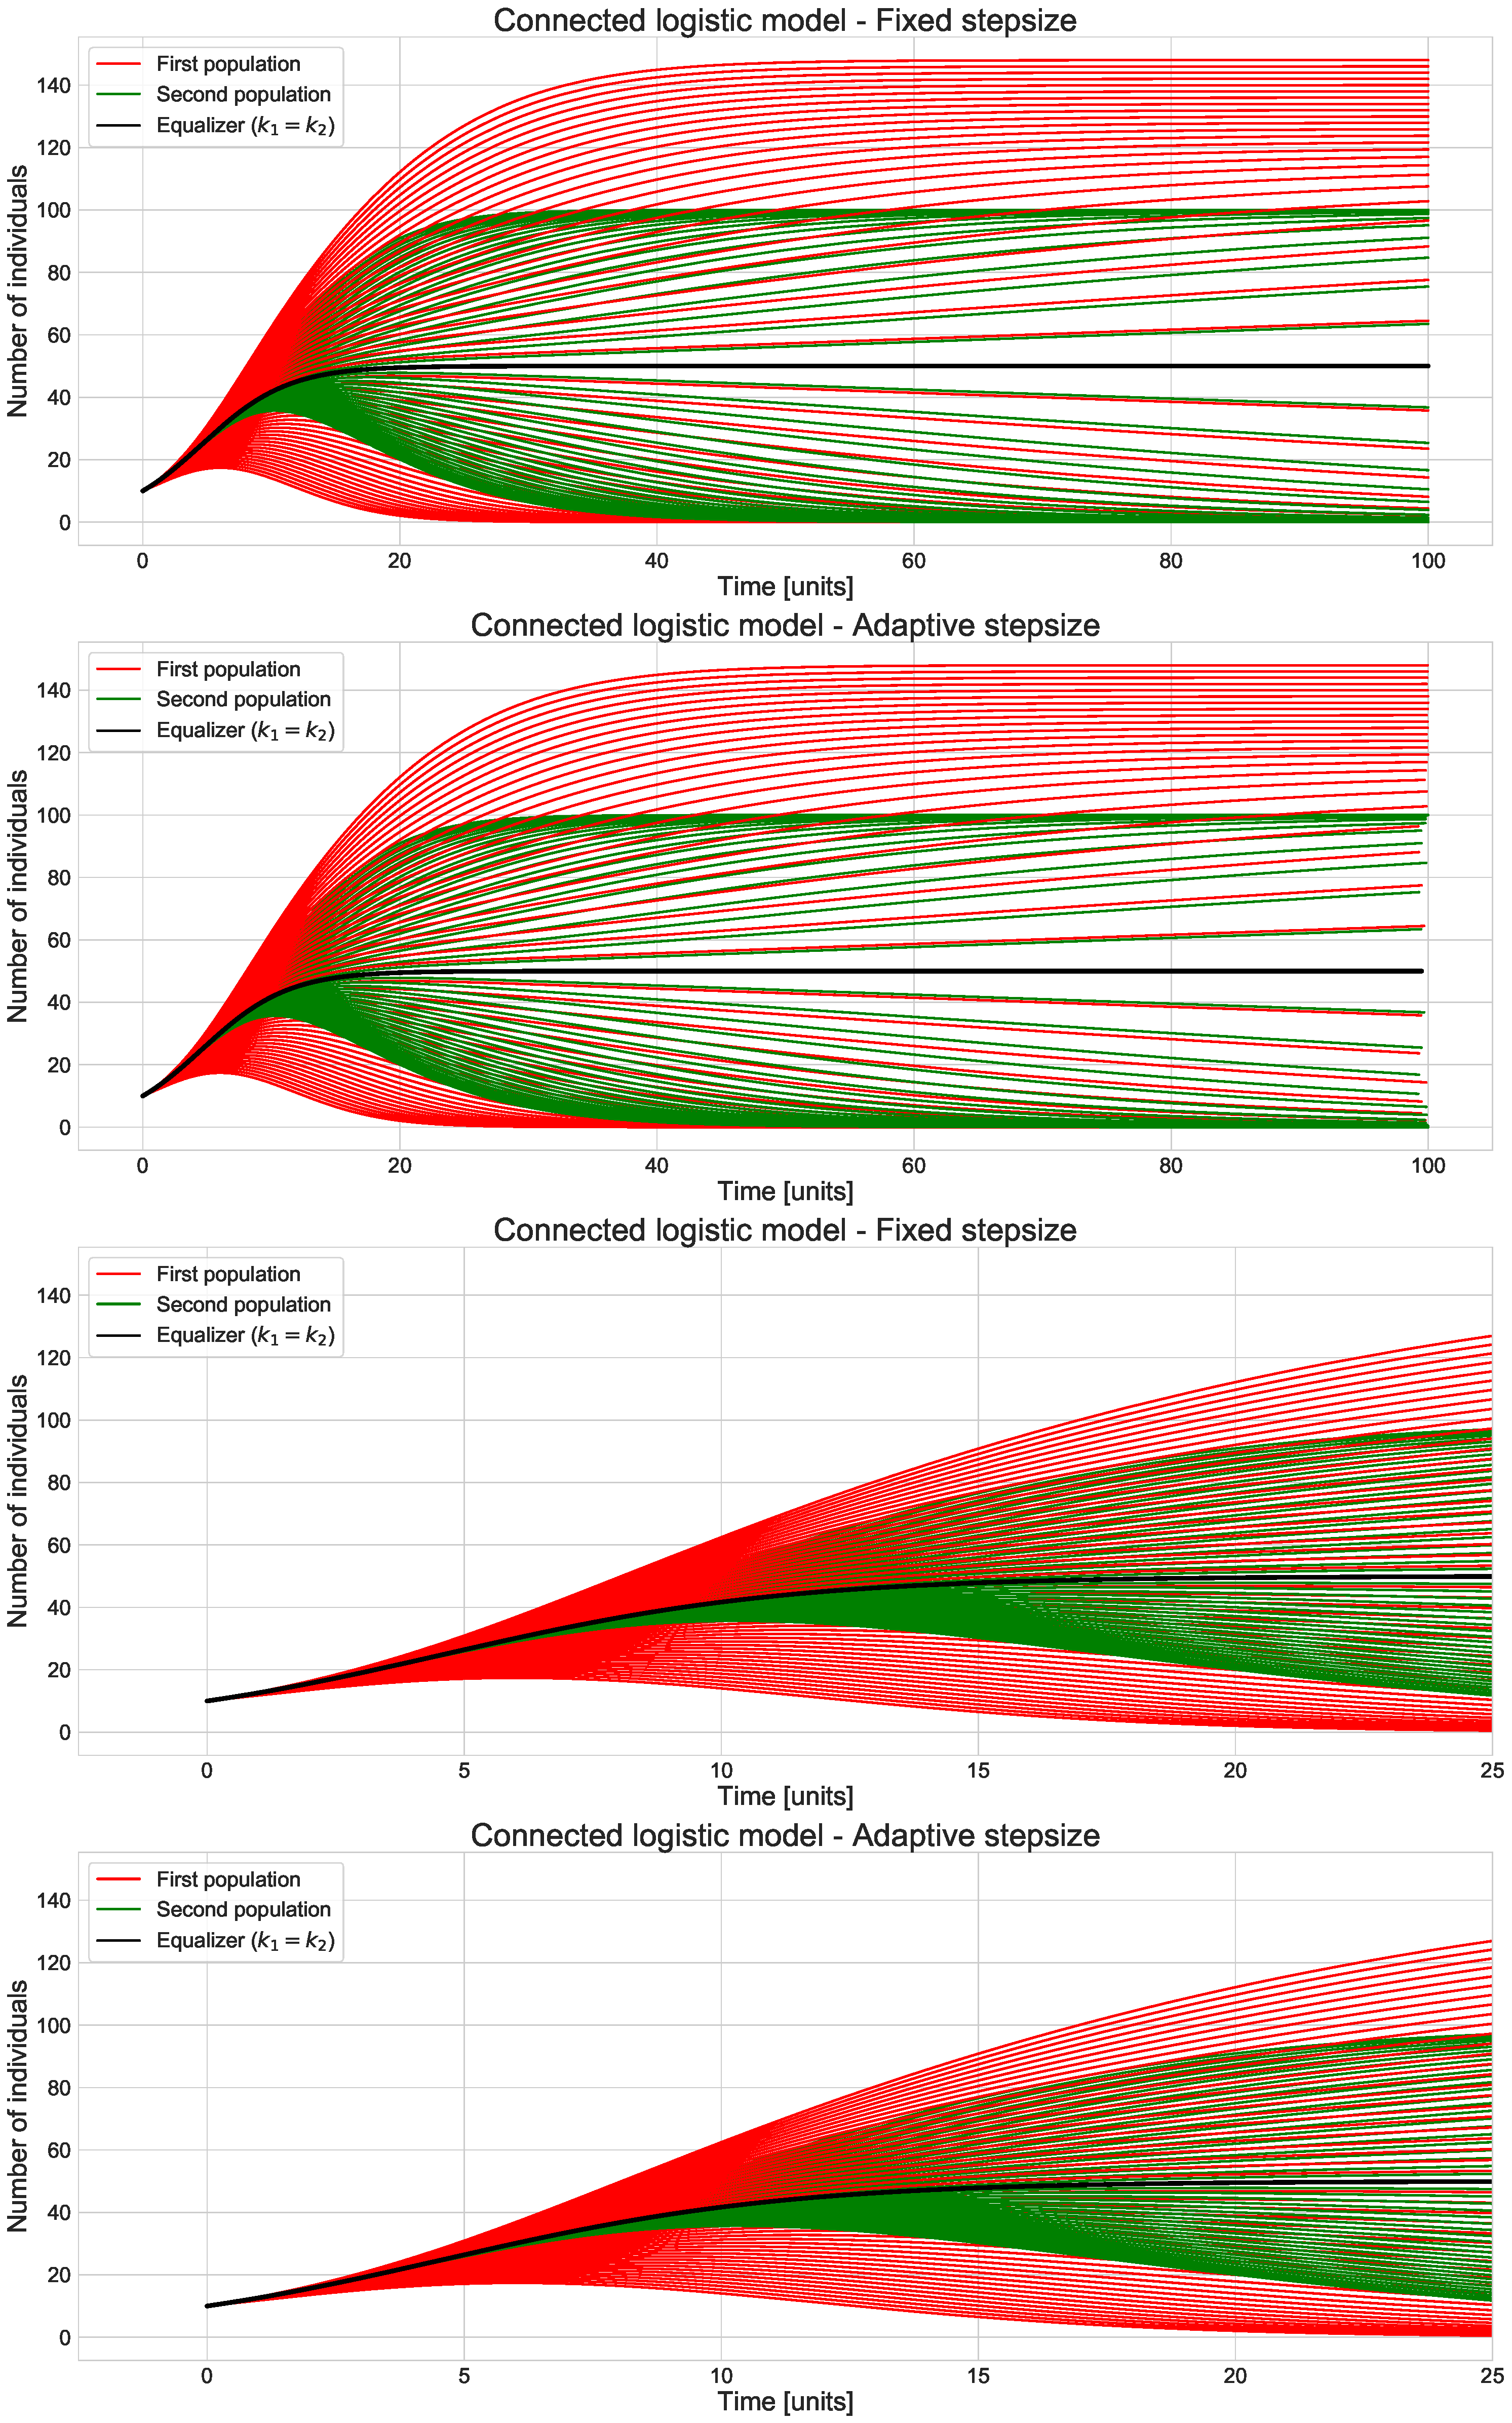
\includegraphics[width=0.92\textwidth]{images/connected_logistic_model_stability.pdf}
    \captionof{figure}{A csatolt-logisztikus modell stabilitásának vizsgálata, $k_{1} \in \left[ 50, 150 \right]$-re, $k_{2} = 100$ maximális egyedszám, $w_{be_{1}} = w_{be_{2}} = 0.6$ születési és $w_{ki_{1}} = w_{ki_{2}} = 0.3$ halálozási ráták, $n_{0_{1}} = n_{0_{2}} = 10$ kezdeti egyedszám, valamint $\alpha = \beta = 1$ kölcsönhatási tényezők mellett. A vastag fekete sáv a $k_{1} = k_{2}$ esetnek megfelelő görbét jelöli, mely esetében a rendszer instabil egyensúlyi helyzetben tartózkodik. A feladatok alapján elemeznünk kellett, hogy igaz-e az állítás, miszerint a nagyobb $k$ paraméterű faj győzedelmeskedik a csatolt-logisztikus egyenlet alapján? Az ábra pontosan ezt a viselkedést próbálja szemléltetni. A $k_{1}$ értéket folyamatosan változtatva $k_{2}$-t szimmetrikusan körbepásztáztam, majd a hozzájuk tartozó görbéket ábrázoltam. Ez alapján kaptam meg a fenti grafikonokat. Ezekről az olvasható le, hogy a $k_{1}$ növelésével a piros (1-es állatfaj) egyre meredekebben nővekedik kezdetben, míg a 2-es állatfaj egyre inkább csökken. Mikor $k_{1}$ érték megegyezik $k_{2}$-vel, a rendszer egyensúlyba kerül, azonban bármerre is mozdul ki onnan, minden esetben divergál. Amíg $k_{2}$ nagyobb értékkel rendelkezik, addig a 2-es populáció száma kovergál a maximumértékéhez, míg az 1-es 0-hoz tart, azonban amint a $k_{1}$ kerekedik felül, a helyzet megfordul. Az alsó két grafikonon a fentiek első negyede van kiemelve.} \label{fig:9}
\end{center}
\vspace*{\fill}
\newpage
\subsection*{A.4.  A csatolt-logisztikus-modell fázisdiagramjai}
\topskip0pt
\vspace*{\fill}
\begin{center}
    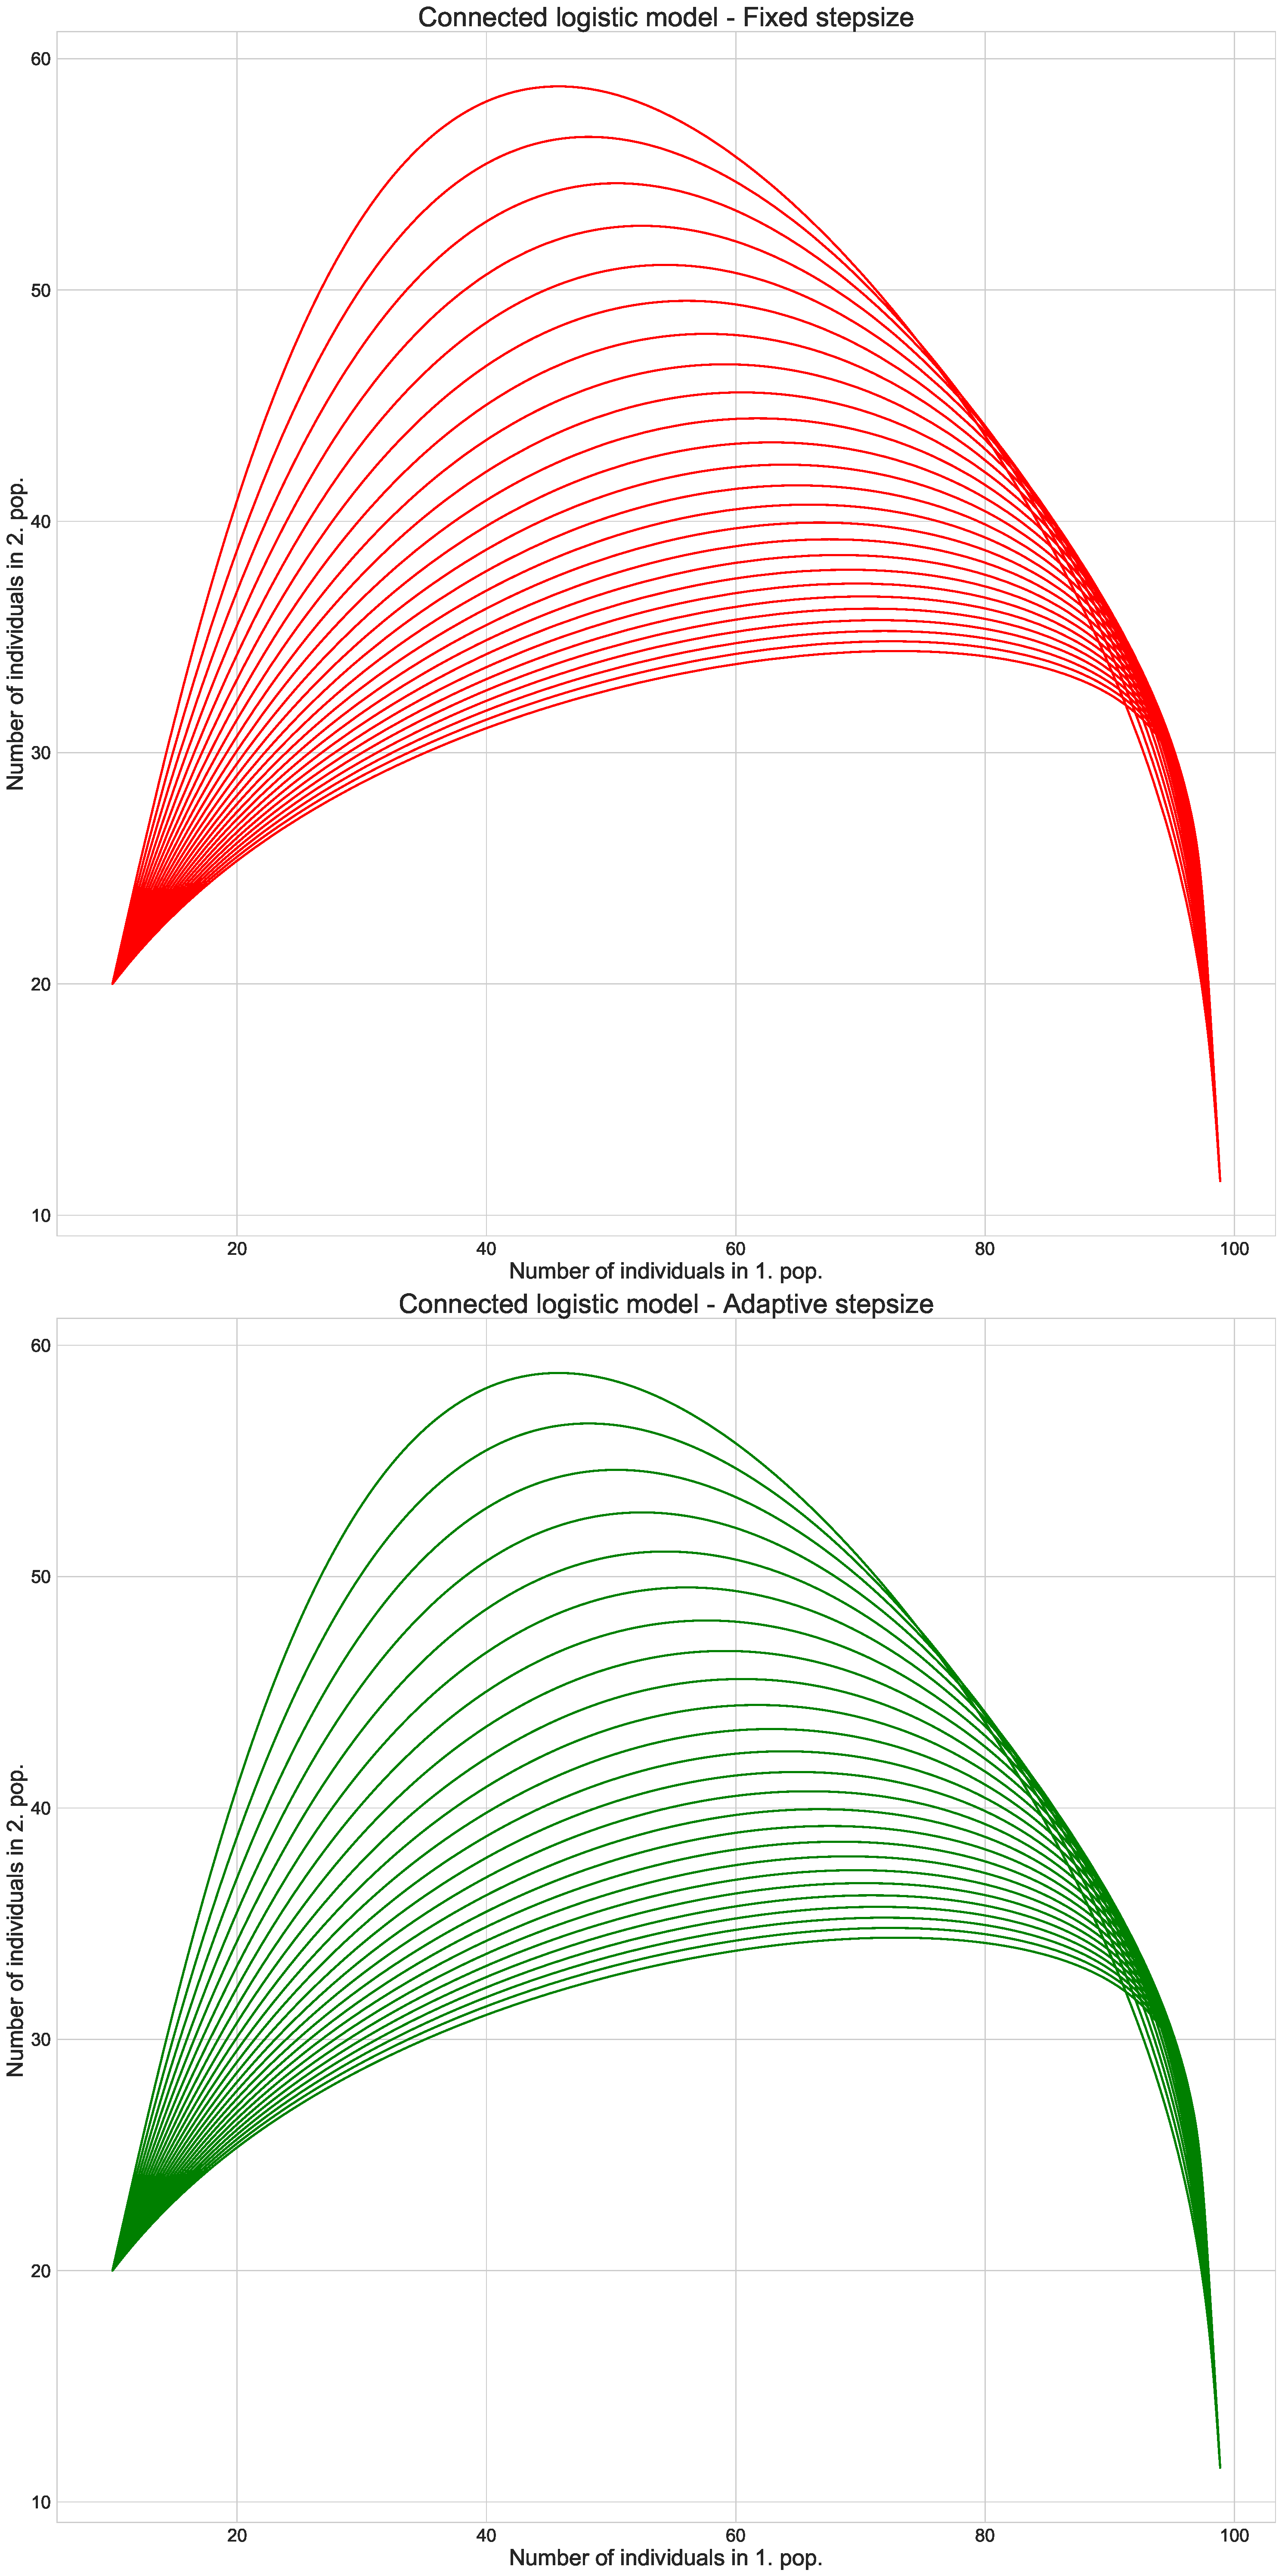
\includegraphics[width=0.80\textwidth]{images/connected_logistic_model_animals.pdf}
    \captionof{figure}{A csatolt-logisztikus modell populációinak változása, $n_{1} - n_{2}$ diagramon ábrázolva, $w_{be_{1}} \in \left[ 0.5, 1 \right]$-re, ahol $w_{be_{1}}$ a sorszám szerinti első faj születési rátája, $w_{be_{2}} = 0.6$ születési, $w_{ki_{1}} = w_{ki_{2}} = 0.3$ halálozási ráták, $n_{0_{1}} = 10$, $n_{0_{2}} = 20$ kezdeti egyedszámok és $k_{1} = k_{2} = 100$ maximális egyedszám, valamint $\alpha = 0.1$ és $\beta = 0.9$ kölcsönhatási tényezők mellett, $\texttt{sim\_time} = 100$ időegység hosszú szimuláció esetén.} \label{fig:10}
\end{center}
\vspace*{\fill}
\newpage
\topskip0pt
\vspace*{\fill}
\begin{center}
    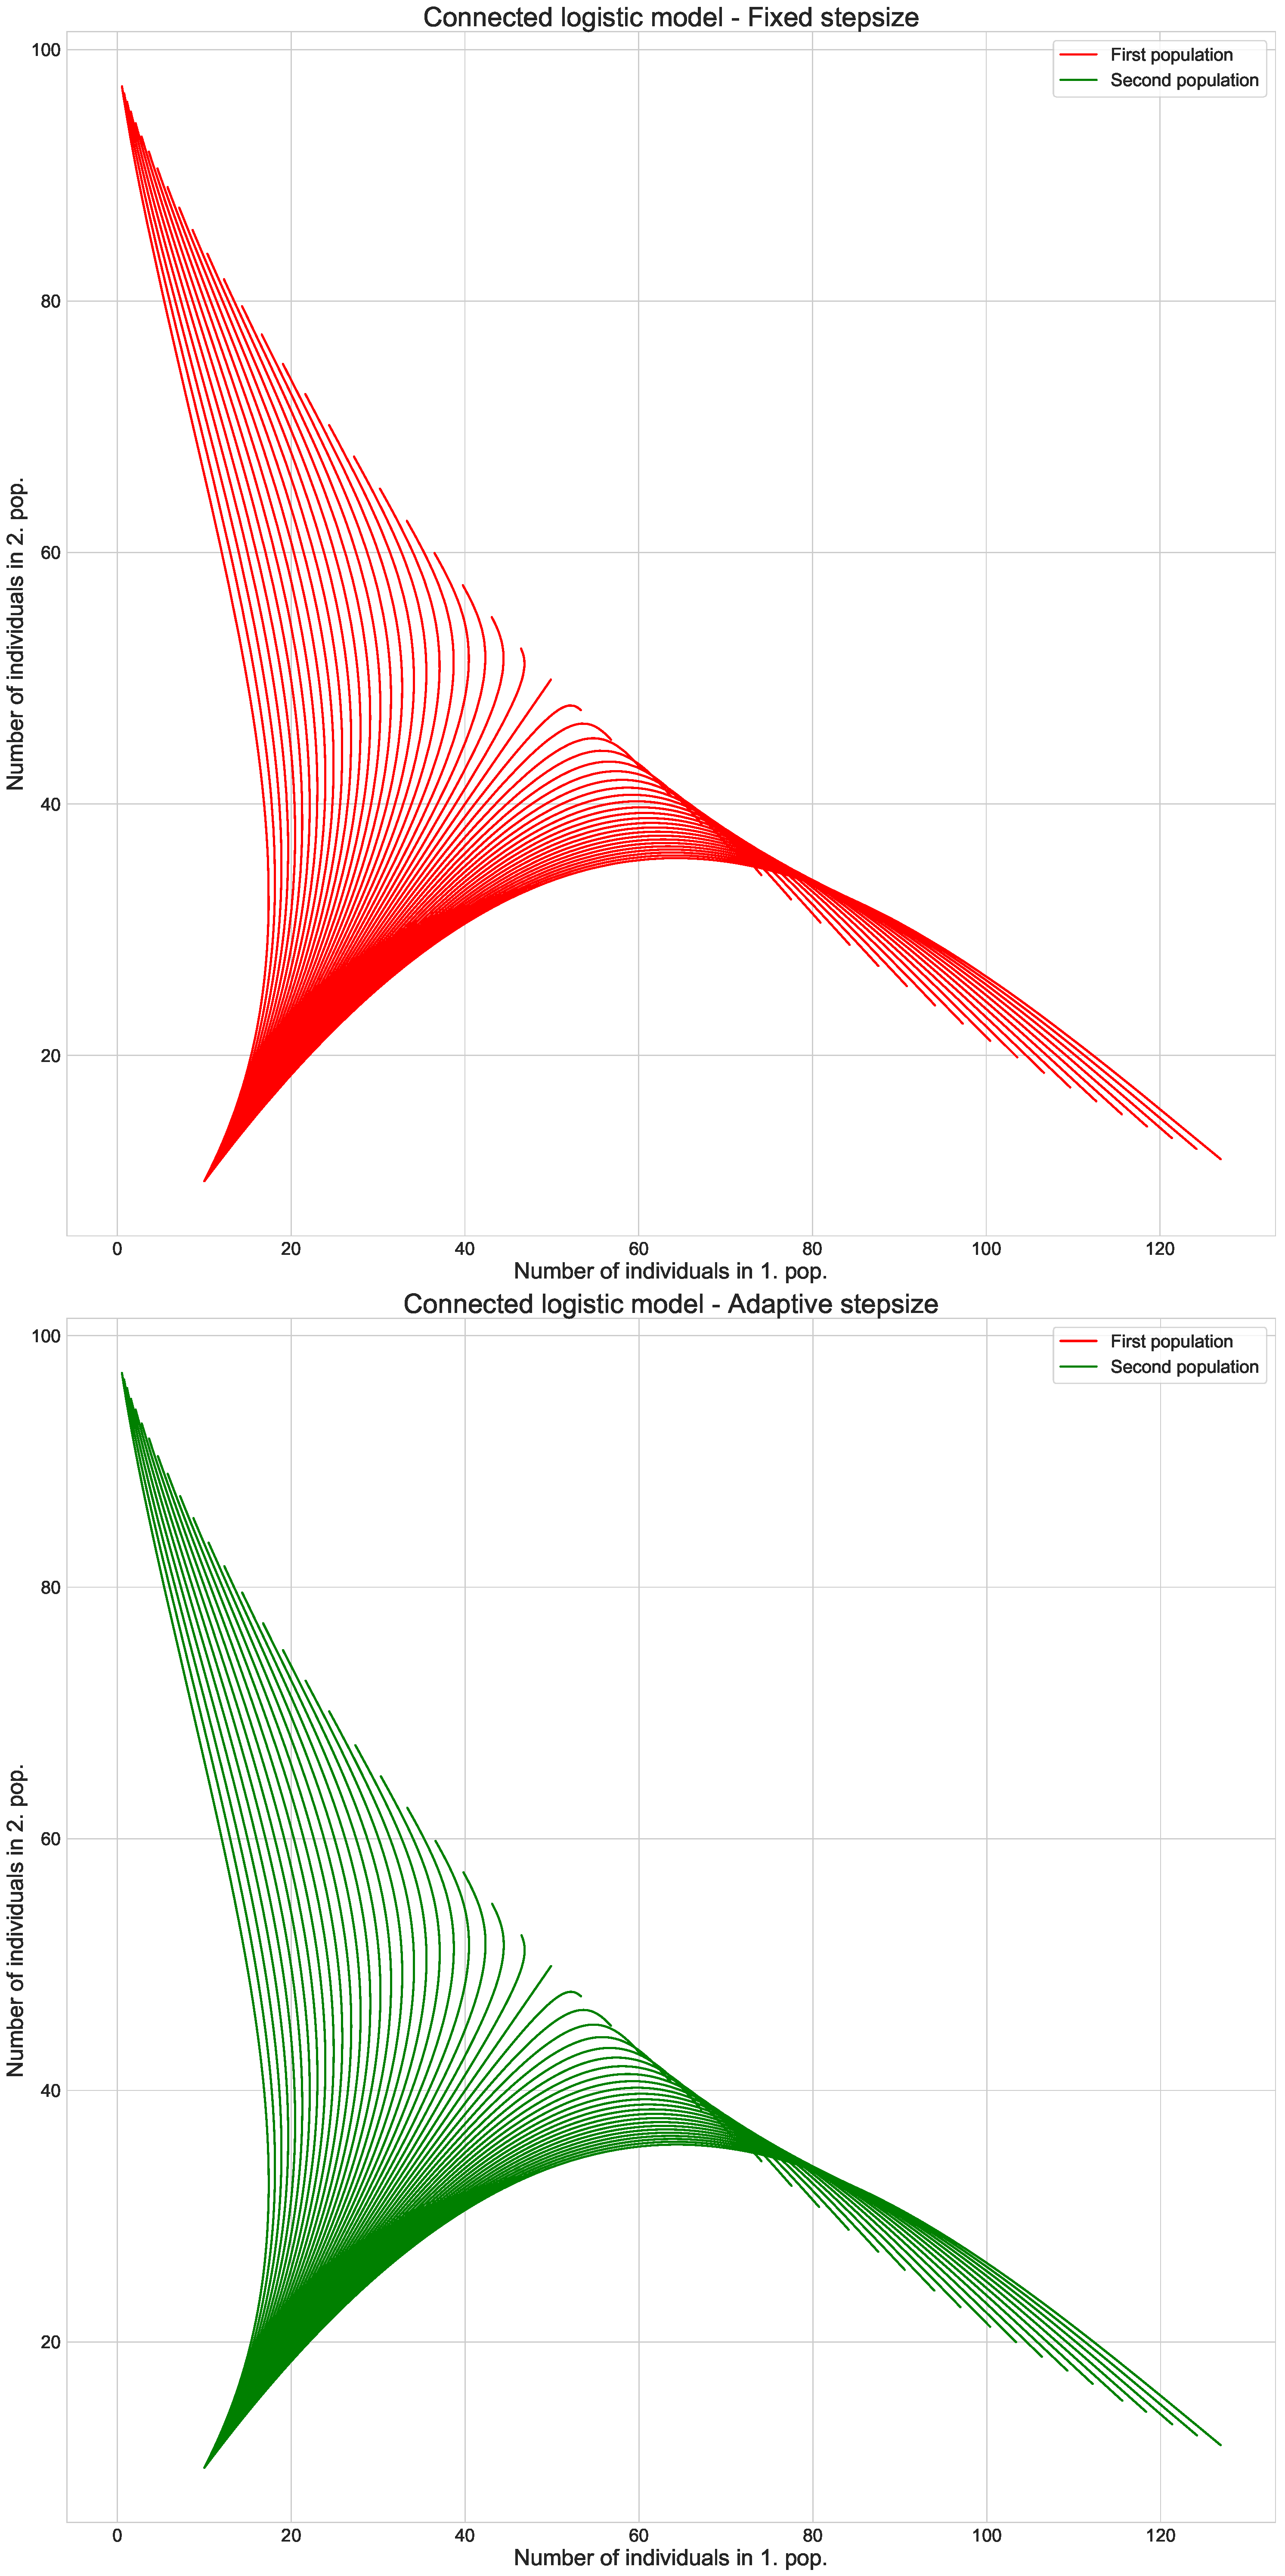
\includegraphics[width=0.81\textwidth]{images/connected_logistic_model_stability_animals.pdf}
    \captionof{figure}{A csatolt-logisztikus modell populációinak változása, $n_{1} - n_{2}$ diagramon ábrázolva, $k_{1} \in \left[ 50, 150 \right]$-re, $k_{2} = 100$ maximális egyedszám, $w_{be_{1}} = w_{be_{2}} = 0.3$ születési és $w_{ki_{1}} = w_{ki_{2}} = 0.3$ halálozási ráták, $n_{0_{1}} = 10$, $n_{0_{2}} = 20$ kezdeti egyedszámok, valamint $\alpha = \beta = 1$ kölcsönhatási tényezők mellett, $\texttt{sim\_time} = 100$ időegység hosszú szimuláció esetén.} \label{fig:11}
\end{center}
\vspace*{\fill}
\newpage
\subsection*{A.5.  A Lotka--Volterra-modell fázisdiagramjai}
\topskip0pt
\vspace*{\fill}
\begin{center}
    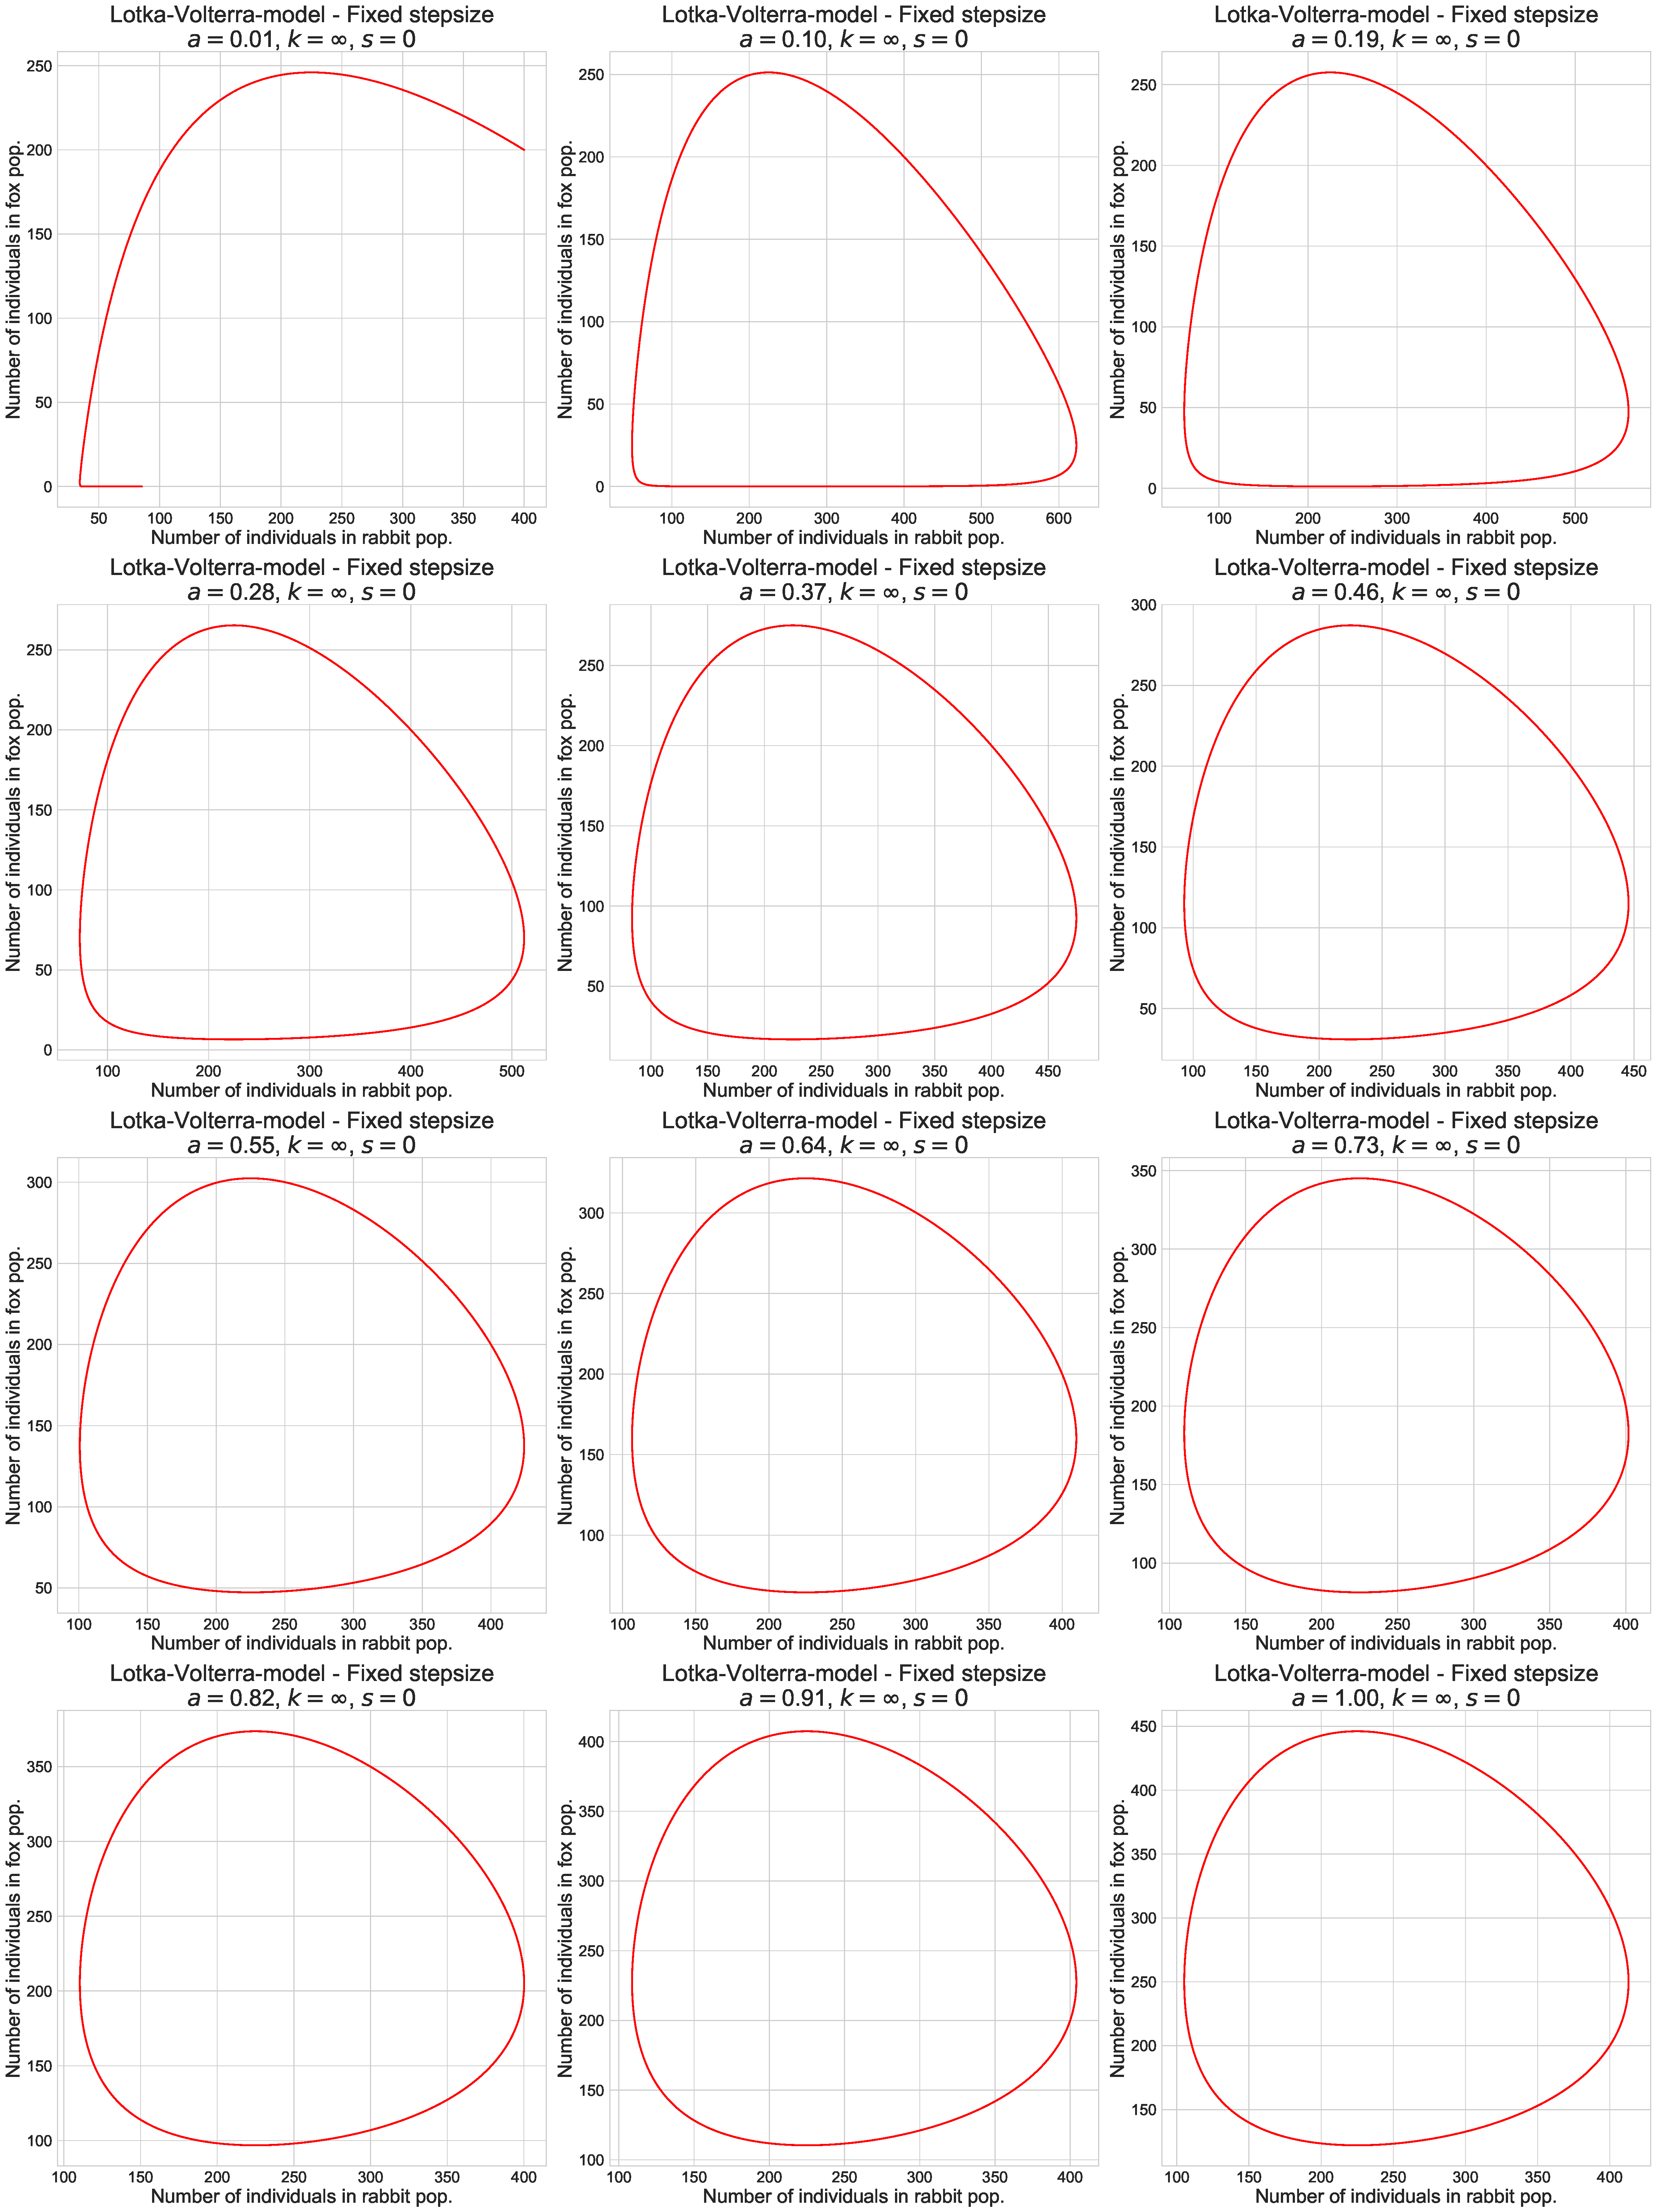
\includegraphics[width=\textwidth]{images/lv_model_animals.pdf}
    \captionof{figure}{A Lotka--Volterra-modell populációinak változása, $n_{r} - n_{f}$ diagramon ábrázolva, $a \in \left[ 0.1, 1.1 \right]$ paraméter esetén, $n_{0_{r}} = 400$, $n_{0_{f}} = 200$ kezdeti egyedszámok, valamint $b = c = 0.004$, $d = 0.9$ fejlődési ráták mellett, $k \to \infty$, $s = 0$ határesetben, $\texttt{sim\_time} = 100$ időegység hosszú szimuláció esetén.} \label{fig:12}
\end{center}
\vspace*{\fill}
\newpage
\topskip0pt
\vspace*{\fill}
\begin{center}
    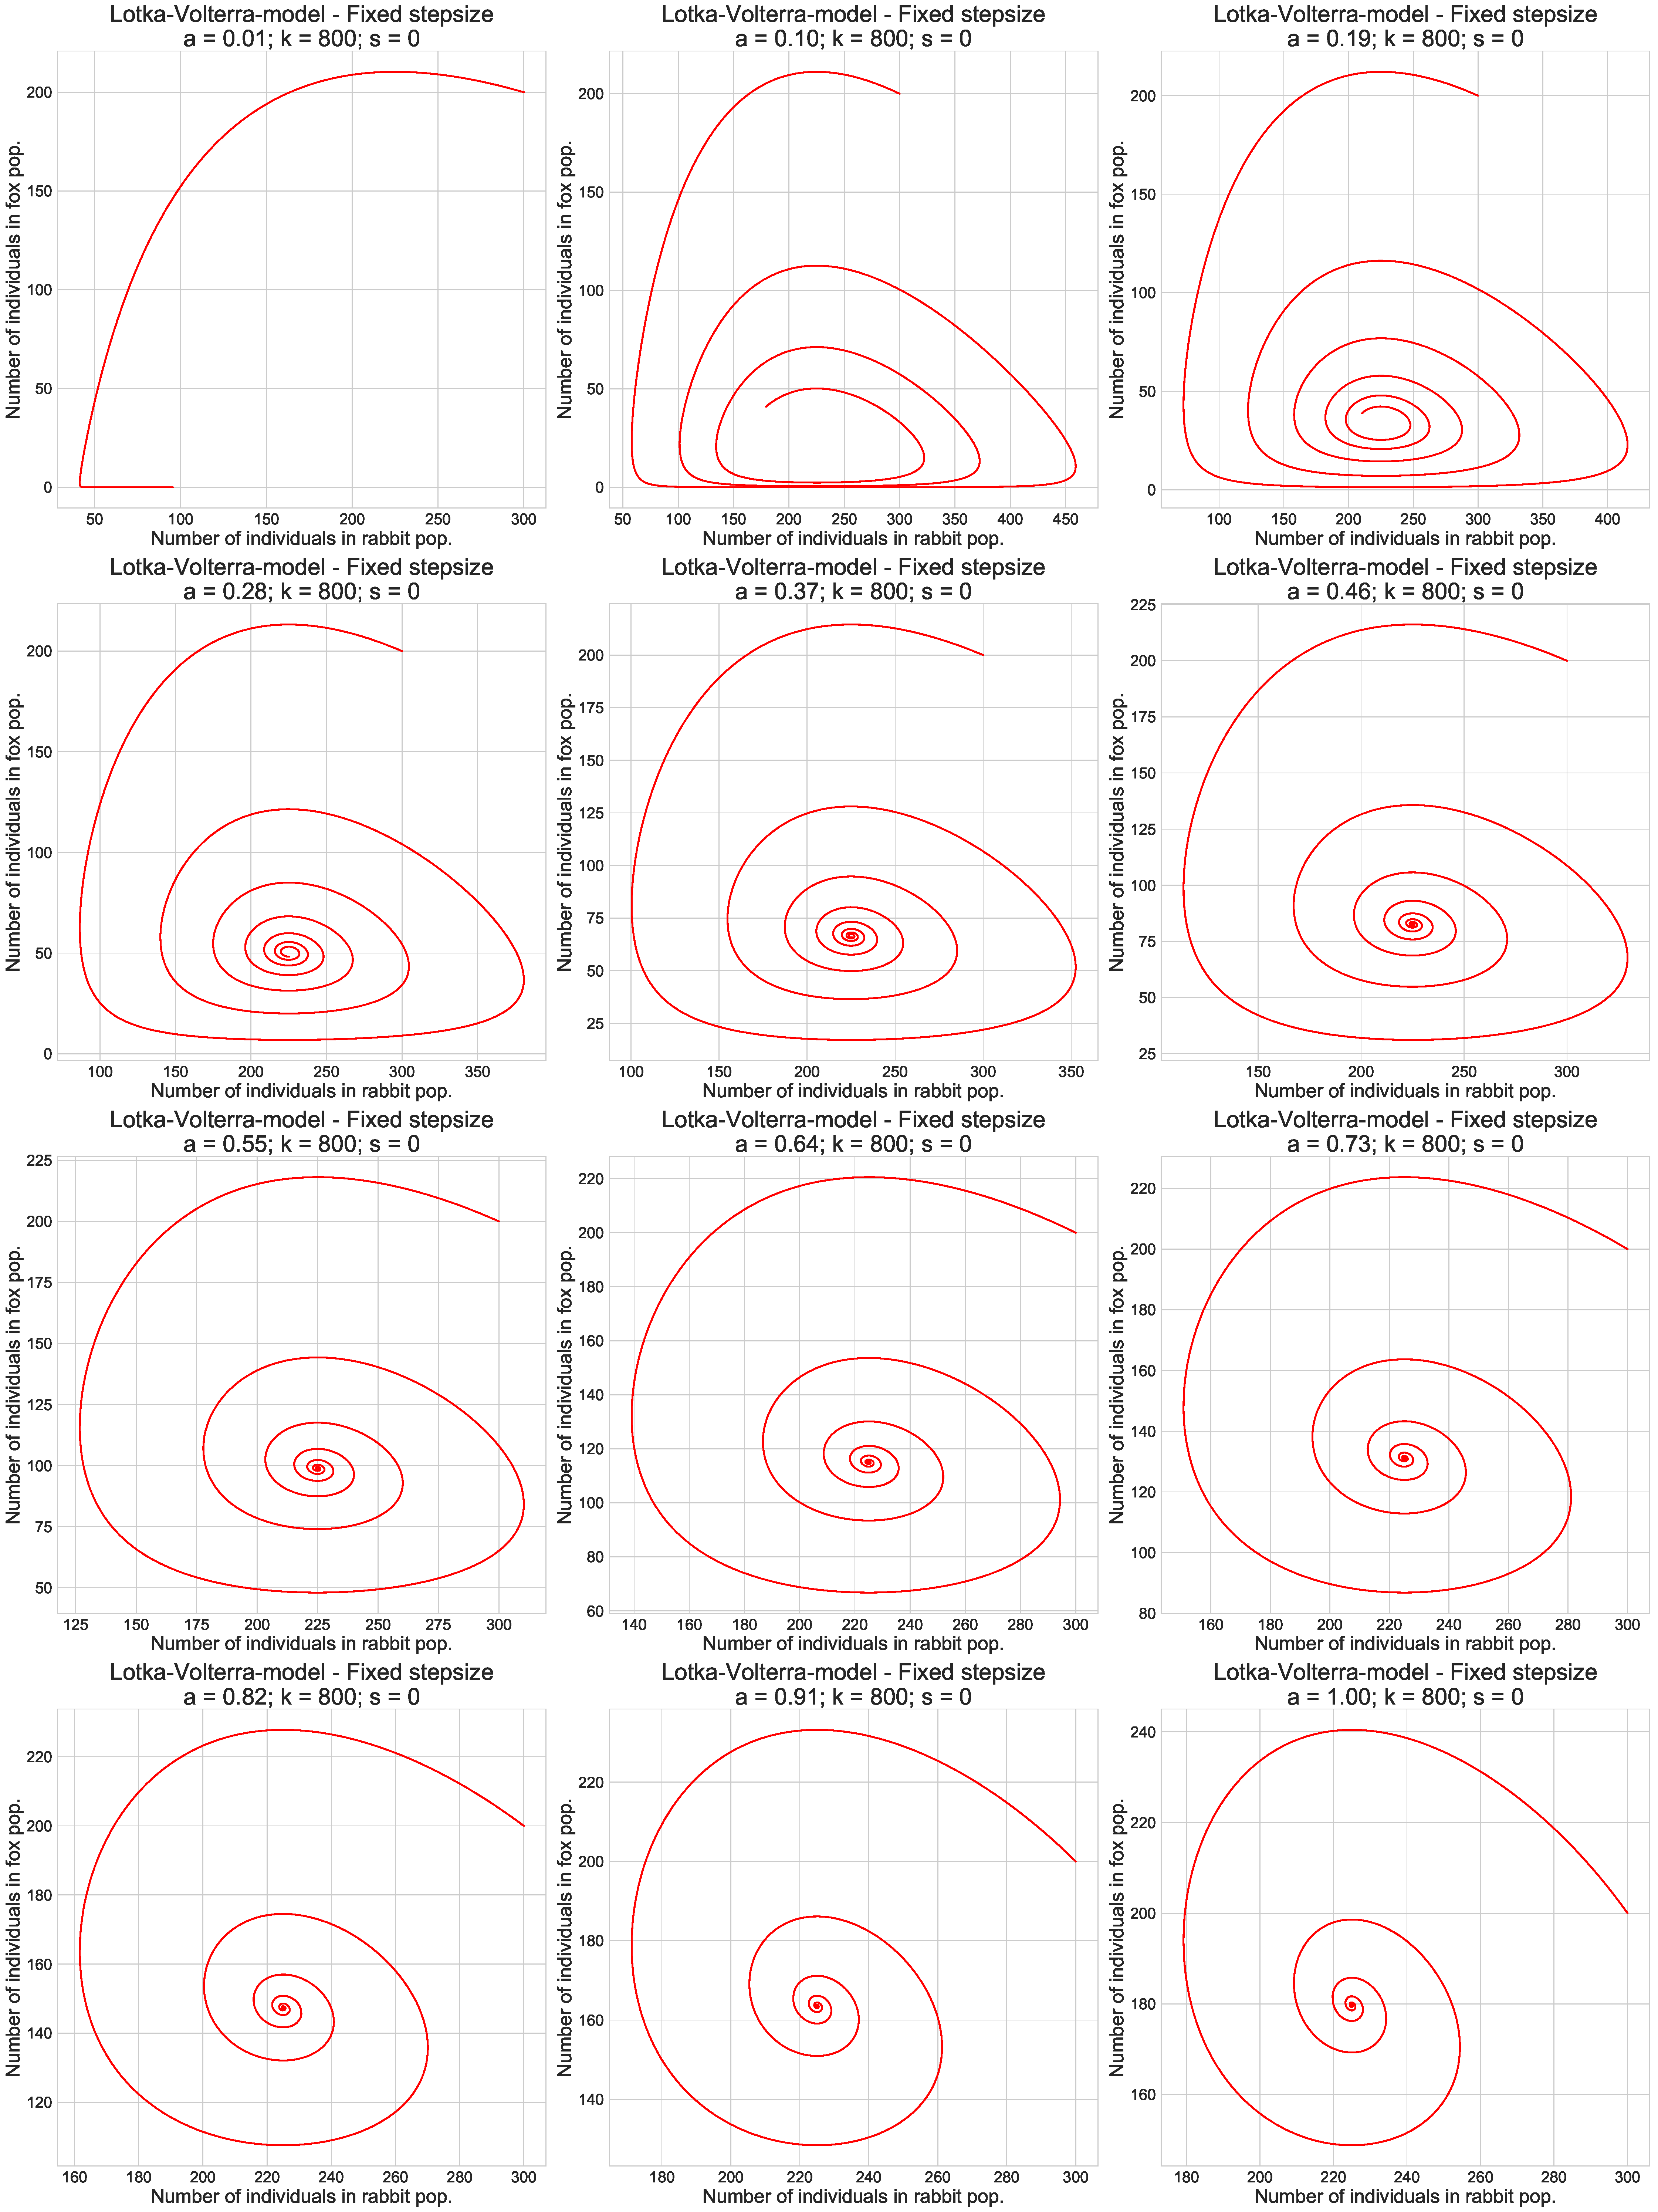
\includegraphics[width=\textwidth]{images/lv_model_drag_animals.pdf}
    \captionof{figure}{A Lotka--Volterra-modell populációinak változása, $n_{r} - n_{f}$ diagramon ábrázolva, $a \in \left[ 0.1, 1.1 \right]$ paraméter esetén, $n_{0_{r}} = 300$, $n_{0_{f}} = 200$ kezdeti egyedszámok, valamint $b = c = 0.004$, $d = 0.9$ fejlődési ráták mellett, $k = 800$, $s = 0$ esetben, $\texttt{sim\_time} = 100$ időegység hosszú szimuláció esetén.} \label{fig:13}
\end{center}
\vspace*{\fill}